%
% The first command in your LaTeX source must be the \documentclass command.
\documentclass[sigchi]{acmart}

%
% defining the \BibTeX command - from Oren Patashnik's original BibTeX documentation.
\def\BibTeX{{\rm B\kern-.05em{\sc i\kern-.025em b}\kern-.08emT\kern-.1667em\lower.7ex\hbox{E}\kern-.125emX}}

% Rights management information.
% This information is sent to you when you complete the rights form.
% These commands have SAMPLE values in them; it is your responsibility as an author to replace
% the commands and values with those provided to you when you complete the rights form.
%
% These commands are for a PROCEEDINGS abstract or paper.
\copyrightyear{2019}
\acmYear{2019}
\setcopyright{acmlicensed}
\acmConference[SNA '21]{Social Network Analysis '21}{2020/21}{University of Pisa, Italy}
\acmBooktitle{Social Network Analysis '21}
\acmPrice{0.00}
%\acmDOI{10.1145/1122445.1122456}
%\acmISBN{978-1-4503-9999-9/18/06}


% end of the preamble, start of the body of the document source.
\begin{document}

%
% The "title" command has an optional parameter, allowing the author to define a "short title" to be used in page headers.
\title{Network analysis of Twitter mentions addressing famous Italian medical scientists}

%
% The "author" command and its associated commands are used to define the authors and their affiliations.
% Of note is the shared affiliation of the first two authors, and the "authornote" and "authornotemark" commands
% used to denote shared contribution to the research.
\author{Francesco Di Cursi, Gennaro Marco Devincenzis}
\email{f.dicursi@studenti.unipi.it, g.devincenzis@studenti.unipi.it}
\affiliation{%
  \institution{Student ID: 625922, NA}
}

\renewcommand{\shortauthors}{One and Two, et al.}


% The abstract is a short summary of the work to be presented in the article.
\begin{abstract}
In the present work we investigate Twitter dynamics during Covid-19 pandemic by selecting those tweets that contains some famous Italian scientist names in a chronological window that goes from the very beginning of January 2020 to the first week of July 2021. We explain how we handled data in order to use mentions as interaction. After this we follow with a statistical description of our network and then we compare our network with different network models. We show different community discovery algorithm and different evaluation strategies, both internal and external. In the same way, we provide different models with regard of spreading topic and different unsupervised alghoritms for link prediction.
Lastly we inspect some of the most interesting results in order to convey a real meaning to these, also by calculating sentiment analysis and its distribution in time. We did this both on general trend and on scientist personal trends. We also provide some wordclouds to help the reader to get a hint of tweet semantics according to sentiment.\footnote{
{\bf Project Repository}
\noindent \url{https://github.com/sna-unipi/2021---final-project-dicursi-devincenzis}}
\end{abstract}




%
% Keywords. The author(s) should pick words that accurately describe the work being
% presented. Separate the keywords with commas.
\keywords{Social Network Analysis, Twitter, SARS-CoV-2, Scientists, Community Discovery, Link Prediction, Sentiment Analysis}


%
% This command processes the author and affiliation and title information and builds
% the first part of the formatted document.
\maketitle

\section{Introduction}
Twitter is a microblogging service (heavily text-oriented), widely used also by prominent individuals in order to convey informations to the masses. It has been created in 2006 by Jack Dorsey and the languages provided were just english and japanese. Furthermore, its limit on each tweet used to be 140 characters. In 2009, the growing attention toward this new service has been leading to a wider spectrum of languages (Italian, French, Dutch and Spanish), allowing Twitter to become the first microblogging service used worldwide in all kind of propaganda, from politics to science. With a further evolution, the limit has been doubled: now a tweet can contain up to 280 characters but this improvement showed little impact on the effective extension of a tweet. In fact, the average length of a tweet has not grown that much (according to Twitter, only 5\% of tweets are longer than 190 characters and, moreover, the most common length has been 34 with the previous limit, and 33 with the new one). The only real difference is a lower use of abbreviation (e.g., "great" instead of "gr8", etc...).

Given Twitter popularity (73.2 million users in April 2021) it is a useful medium to study user interactions and their polarization on matters of public interest. This can be easily done by using each account as node and choosing another parameter as link (it could be the reply or the mention to someone or the hashtags used in the tweet). By doing this, niches can be traced along their respective hubs. Most importantly, characteristics that are hidden in peaceful times usually emerge during crises, giving an optimal context for analysis.


The aim of this paper is to inspect the impact of Covid-19 pandemic on the media attitude to build customer loyalty through "testimonial" mechanism. Moreover, we want to understand who between these 13 illustrious scientists has been accumulating more fame than others, turning them basically into influencers (thus, using the pandemic as a fame catalyst). Of course, one might say, there are always influencing personalities, but the difference stands in how the discourse is carried on. The idea of this paper, thus, is to investigate the deterioration of the scientific discourse by virtue of the pauperization of the content of the message in favour of its virality, in what resembles a "war to the last tweet". As a matter of fact, some scientists have been communicating improperly, making the same mistakes of those who they have been \textit{'blasting'}(i.e., speaking with too much emphasis, and even insulting others, on the basis of no unshakable truth while complaining about the same thing when speaking about others with different ideas, scientists or not). In this sense some of them display the same communicational restlessness driven by the same aspiration of those who are in the star-system: in good or bad means, the essential is to be on the mouth of everybody.


\section{Data Collection}
Our study has been conducted by scraping tweets made in time of pandemic and containing the names of 13 well-known Italian scientists. Due to the size of the original dataset, some smaller datasets have been derived from the original one to make the analysis possible with our computational means.

\subsection{Selected Data Sources}

All the tweets scraped have been produced between 2020/01/01 and 2021/07/07, containing the following names:
\begin{itemize}
    \item Alberto Zangrillo
    \item Andrea Crisanti
    \item Fabrizio Pregliasco
    \item Ilaria Capua
    \item Massimo Galli
    \item Matteo Bassetti
    \item Nino Cartabellotta
    \item Pier Luigi Lopalco
    \item Roberto Burioni
    \item Robert Gallo
    \item Roberto Gualtieri
    \item Silvio Brusaferro
    \item Walter Ricciardi
\end{itemize}
Between these 13 individuals, as it will be shown, just 2 of them have effectively polarized the pandemic discourse, thus configuring themselves as hubs.


\subsubsection{Crawling Methodology and Assumptions}

The present study has been conducted by scraping tweets with 13 relevant names in the Italian scientific landscape, from 2020/01/01 to 2021/07/07.For each tweet we have extracted the following information:
\begin{itemize}
    \item created$\_$at: a complex piece of information made by date, time and continent;
    \item 'date': the date in which the tweet has been made;
    \item 'time': time at which the tweet was posted;
    \item 'id': identification code of the individual making the tweet;
    \item 'username': his username;
    \item 'mentions': individuals who have been mentioned;
    \item 'tweet': content of the tweet;
    \item 'language': author's language;
    \item 'hashtags': hashtags used in the tweet;
    \item 'replies$\_$to': individuals to whom the author replies to;
    \item 'replies$\_$count': number of replies to the tweet;
    \item 'retweet': whether the tweet has retweets or not;
    \item 'retweets$\_$count': number of retweets.
\end{itemize}

In order to trace interactions, we derived a mention-only dataset. The retrieved columns are the following:
\begin{itemize}
    \item 'created$\_$at'
    \item 'date'
    \item 'time'
    \item 'id'
    \item 'username'
    \item 'mentioned$\_$id': the author's identification code;
    \item 'screen$\_$name': the username of the mentioned user;
    \item 'tweet'
    \item 'language'
    \item 'hashtags'
    \item 'replies$\_$count'
    \item 'retweet'
    \item 'retweets$\_$count'
    \item 'conversation$\_$index': the index of each row of the mention-filtered dataset, in order to keep track of the conversation (if the author mentions more than one individual in the same tweet);
\end{itemize}


\section{Network Characterization}
We decided to use a graph where the links are the mentions between users. Our graph has 34,714 nodes with 75,653 links. The graph being weighted, some of those links have weight $>= 1$, corresponding to multiple mentions to the same node. For data analysis we decided to use Python (and the Networkx library). We used Gephi for a visual representation.

\begin{figure}[htbp!]
    \centering
    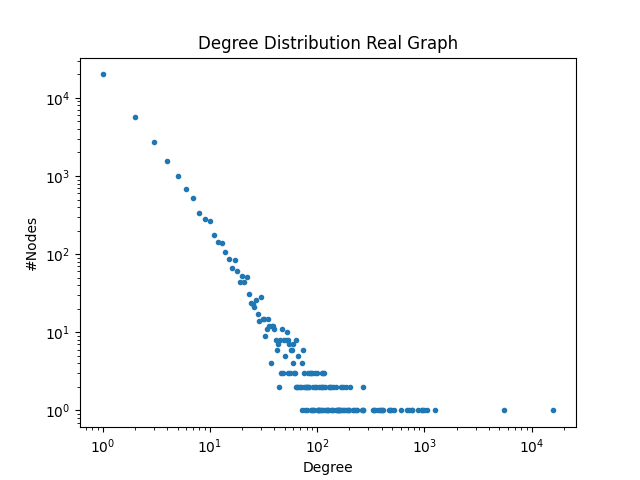
\includegraphics[width=0.5\textwidth]{img/degreeDistRealGraph.png}
    \captionof{figure}{Degree distribution of our graph}
    \label{fig:my_label}
\end{figure}

\begin{figure*}[htbp!]
\centering
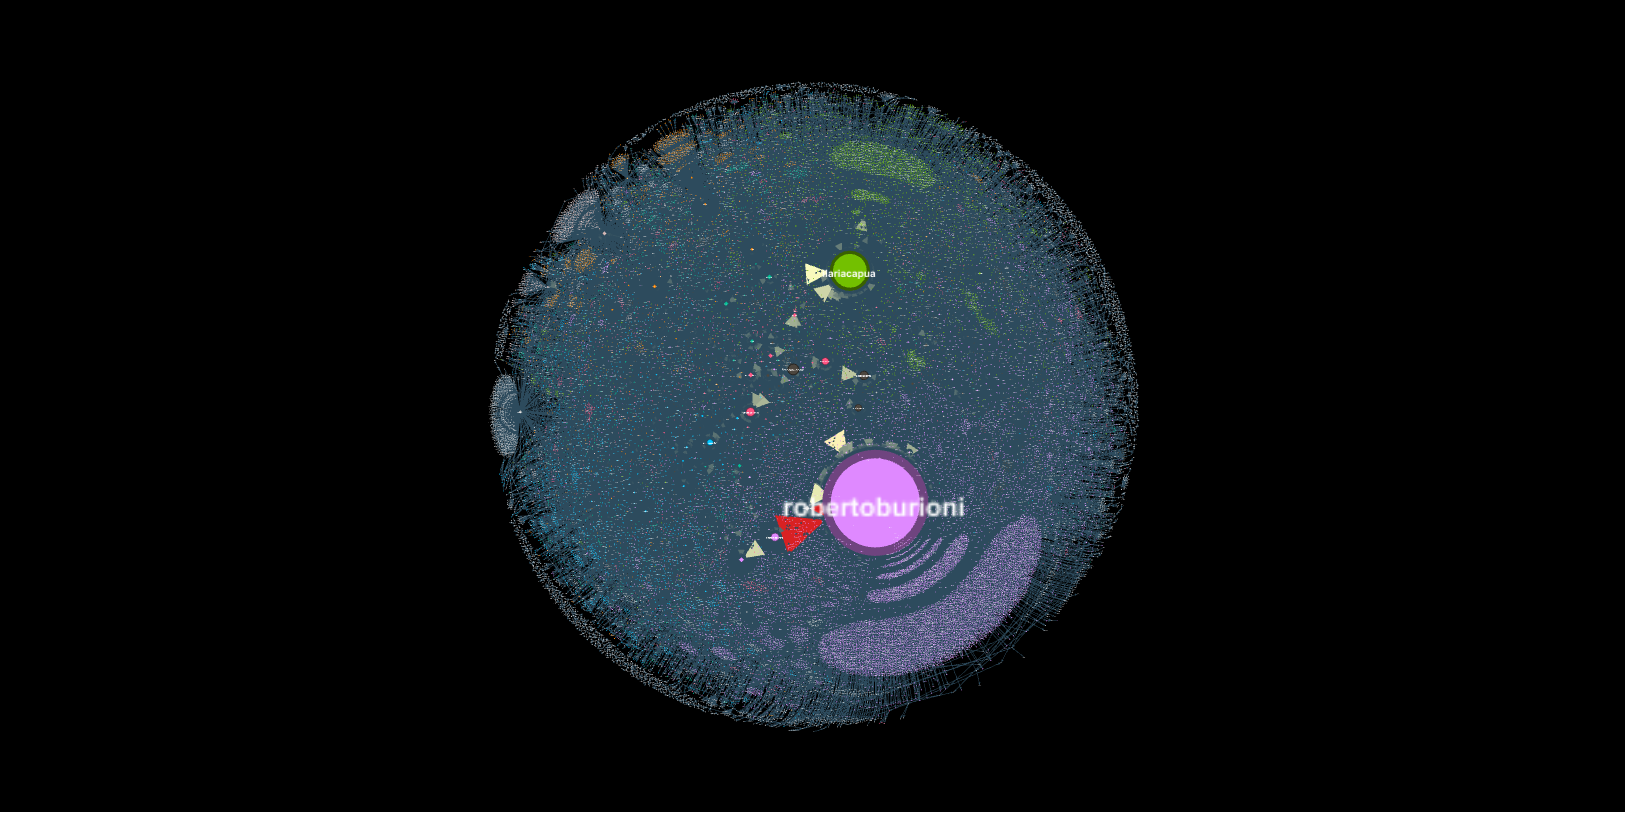
\includegraphics[width=\textwidth]{img/Results/wigthedInOut.png}
\captionof{figure}{Gephi ForceAtlas2 layout, strong gravity; node and text size according to weighted degree, node colors according to modularity, edge colors (from blue to red) according to weight.}
\end{figure*}

\subsection{Statistics of our graph}
\subsubsection{Degree distribution}
We plotted the degree distribution of our network, obtaining a line in log-log scale, meaning that it is roughly a power law. This is consistent with the fact that there are few nodes with disproportionately high degree. A maximum likelihood estimation of a power law returns $\gamma = 2.39$. The average degree of our graph is 2.18 and the average weighted degree 4.36.

\subsubsection{Centrality analysis}
We calculated, for our graph, several centrality measures, agreeing most of the times with our expectations: the most central nodes were either VIPs, newspapers or TV stations or the names we selected in the beginning for filtering.
We follow with a list of the most central nodes according to each measure. \\
Eigenvector centrality
\begin{enumerate}
    \item ilariacapua - 0.5183829888462345
    \item robertoburioni - 0.29280538629366504
    \item corriere - 0.11000142565126599
    \item onehealthuf - 0.091722716788958
    \item chetempochefa - 0.09025499776506105
    \item la7tv - 0.08630786403397056
\end{enumerate}

PageRank
\begin{enumerate}
    \item ilariacapua - 0.14805560924351835
    \item robertoburioni - 0.1237508731759336
    \item onehealthuf - 0.023338855487779718
    \item chetempochefa - 0.015592779209953066
    \item medicalfactsit - 0.011548756666784864
    \item azangrillo - 0.010157518029303338
\end{enumerate}

Closeness centrality
\begin{enumerate}
    \item robertoburioni - 0.47393835471776397
    \item ilariacapua - 0.3399676198772533
    \item chetempochefa - 0.29674367558206
    \item azangrillo - 0.27613466686929616
    \item medicalfactsit - 0.2740243480799648
    \item corriere - 0.23009079952159298
\end{enumerate}

Harmonic centrality
\begin{enumerate}
    \item robertoburioni - 18741.145634919543
    \item ilariacapua - 13264.996067822003
    \item chetempochefa - 10846.996067822425
    \item azangrillo - 10100.379401157166
    \item medicalfactsit - 10065.146067823993
    \item corriere - 8541.990115436854
\end{enumerate}

\subsubsection{Clustering coefficient and density analysis}
We computed the average clustering coefficient of our network, and it came out to be $0.082$. The density on the other hand came out to be $6.28\cdot10^{-5}$. This value is such a small number mainly for two reasons, which are the fact that in most real life networks existing links are a small fraction of possible links and the very nature of our graph: most tweets in general have no mention, so the small number is quite natural.
\subsubsection{Connected components analysis}
Our graph, when taken as an undirected graph, has 660 (weakly) connected components. This, again, agrees with the a priori observation that mentions are fairly rare and thus most nodes are disconnected.
\subsubsection{Path analysis}
Our graph has a diameter of 20 (excluding nodes with infinite distance) and an average path length of 5.
\subsection{Comparison with an Erdos-Renyi Random Graph}
Using the $G(N,L)$ definition of an Erdos-Renyi \cite{erdosrenyi} Random Graph, we built a graph with the the same number of nodes and links of our own.
\subsubsection{Degree distribution comparison}
While clearly the mean degree is the same (the reason being that the graph has the same number of nodes and links as our graph) the distribution is wildly different. In loglog scale, the degree distribution of the ER graph has no resemblance to a line; this is consistent with the theoretical fact that its distribution is a Binomial distribution and for a large number of nodes can be approximated by a Poisson distribution.
\subsubsection{Clustering coefficient and density comparison}
For the same reason the average degree is the same as the real graph, the density does not change either. However, the average clustering coefficient is very different, being $3.73\cdot 10^{-5}$. This is consistent with the consideration that the ER random graph does not reproduce the high clustering coefficient of real graphs.
\subsubsection{Connected Component comparison}
The ER graph has 467 connected components, a number that is different from the real graph but of the same order of magnitude.
\subsubsection{Path analysis}
The diameter of the ER graph is 31, while the average path length 12.8. Again, the fact that both of these measures are smaller than the real graph is expected since links are completely random.

\begin{figure*}[!htbp]
    \centering
    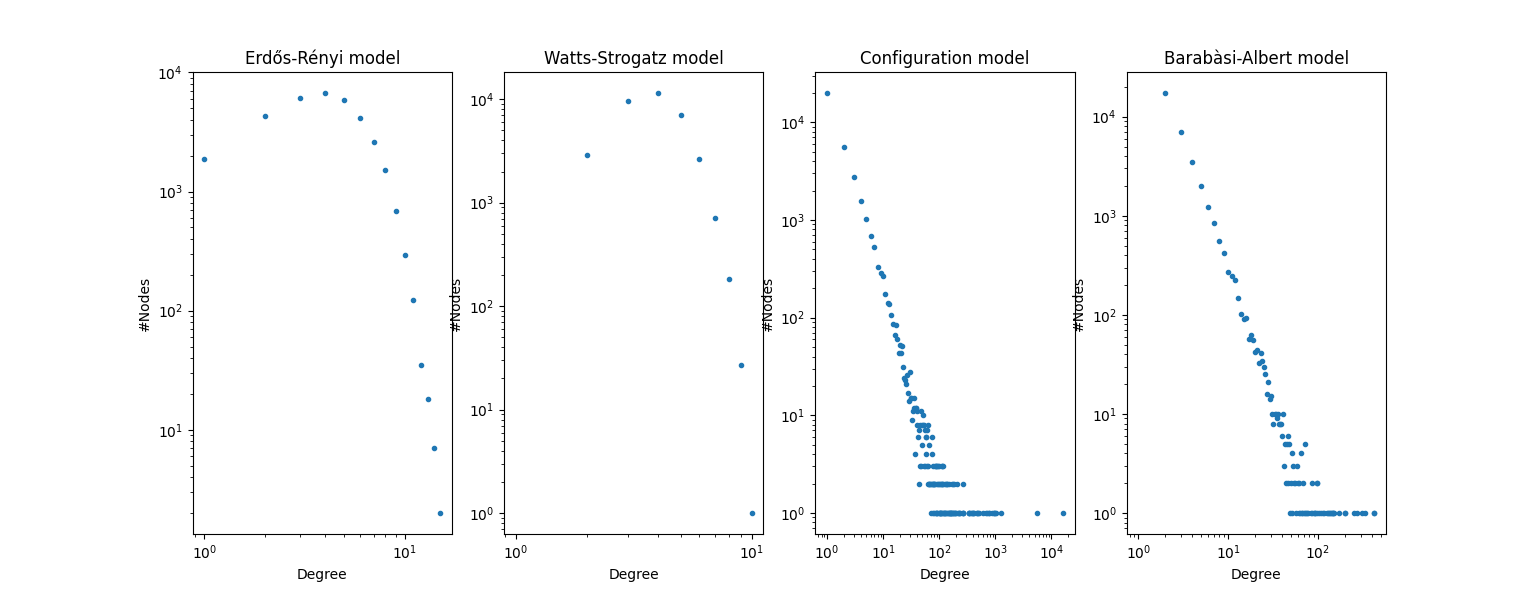
\includegraphics[width=\textwidth]{img/comparisonDegreeDist.png}
    \caption{Degree distribution of comparison graphs}
    \label{fig:my_label}
\end{figure*}

\subsection{Comparison with a Watts-Strogatz model}
We built a Watts-Strogatz\cite{wattsstrogatz} model by choosing the parameter $K$ in such a way to have a similar number of links between nodes: we chose $K=5$, which yields the same number of nodes as the real graph with 69,428 links. As for the rewiring probability, we chose $p=0.47$: this number was chosen to make the clustering coefficient similar to the original graph (since the main advantage of this model over an ER graph is making the clustering coefficient more realistic).
\subsubsection{Degree distribution comparison}
As expected because of theoretical considerations, the degree distribution has the same shape of that of the Erdos-Renyi graph.
\subsubsection{Clustering coefficient and density comparison}
As mentioned in the beginning, the parameter $p$ was chosen for the purpose of making the two clustering coefficients agree: in the Watts-Strogatz graph it is 0.081. The density, since we chose the parameter $K$ to make the number of nodes and links agree, is also very similar.
\subsubsection{Connected Component comparison}
There is only 1 connected component in the network.
\subsubsection{Path analysis}
The diameter of the WS network is 14, while the average path length is 8.80.

\subsection{Comparison with Configuration Model}
We built a directed Configuration Model with the in and out degree sequences of our original graph, ignoring weights.
\subsubsection{Degree distribution} The degree distribution is the same as the original graph by construction.
\subsubsection{Clustering coefficient and density comparison}
The clustering coefficient of the Configuration Model comes out to be 0.032, which is smaller than our original graph but orders of magnitude higher than an Erdos Renyi graph. The density, depending only on number of nodes and links, is the same as the original graph.
\subsubsection{Connected Component comparison}
There are 1252 connected components in the Configuration model we built.
\subsubsection{Path analysis}
The diameter of the CM network is 18, while the average path length is 5.73. Both numbers are similar to the original graph.

\subsection{Comparision with Barabasi Albert model}
We built a Barabasi Albert \cite{barabasialbert} model with the same number of nodes as our original graph and 69424 links.
\subsubsection{Degree distribution} As per theory, the degree distribution is a Power Law with exponent $\gamma = 3$.
\subsubsection{Clustering coefficient and density comparison}
The clustering coefficient of the Barabasi Albert model we built is 0.002, much smaller than the one of the original graph. The density, being the Barabasi Albert graph we built undirected, is double that of our graph (by definition).
\subsubsection{Connected Component comparison}
The BA graph we built has 1 connected component.
\subsubsection{Path analysis}
The diameter of the BA network is 10, while the average path length is 5.513. Both numbers are similar to the original graph.




\section{Task 1: Community discovery}

To discover communities in our graph we decided to use some well known algorithms \cite{barabasiCh9}, namely:
\begin{enumerate}
    \item Angel: This algorithm belongs to the percolation family of community discovery algorithms. It works by considering the ego network (i.e. the network of the neighbours) of a given node, removing the node from it and by performing a label propagation. Once this is done, the "ego node" is inserted in each of the found communities; once this process is performed for all nodes the communities are merged, meaning that communities that have a certain percentage of common nodes are merged into one.
    \item Label Propagation: This algorithm belongs to the percolation family of community discovery algorithms. The label propagation algorithm works by assigning an initial label to some nodes and by propagating them, meaning that each node takes the label of the majority of its neighbours. The algorithm stops when each node has the same label as the majority of its neighbours.
    \item Louvain: This algorithms uses the density definition of communities (communities are a set of densely connected nodes). The Louvain algorithm works by maximizing a measure called modularity, namely:
    $$Q = \frac{1}{2m}\sum_{i,j}\bigg(A_{ij}-\frac{k_i k_j}{2m}\bigg)\delta(c_i,c_j)$$
    Where
    \begin{enumerate}
        \item $m$ is the sum of the weights of all edges
        \item $A_{ij}$ is the element $i,j$ of the adjacency matrix
        \item $c_{i/j}$ are the communities of the nodes
    \end{enumerate}
    This is done in a two step process, where in the first step a certain node is inserted in the community that guarantees the biggest increase in modularity, while in the second step an aggregation of the network is performed and the first step is repeated in the aggregated network.
    \item Walktrap: This algorithm works by leveraging the fact that random walks on a graph tend to get trapped inside a community.
\end{enumerate}
For this task we ignored the original directedness of our graph. We decided to evaluate the algorithms in two ways: using internal evaluation strategies and external evaluation strategies. As for internal evaluation strategies, we decided to calculate the following quality measures
\begin{enumerate}
    \item Average Internal Degree (AID): the average degree of the communities considering only edges inside the community;
    \item Internal Density (ID): The internal density of the community;
    \item Girvan Newman Modularity (GNM): $Q$ as explained in the Louvain algorithm
    \item Conductance: The fraction of total edge volume that points outside the algorithms
    \item Node coverage: Fraction of nodes that is inside a community
    \item Triangle Participation Ratio (TPR): is the fraction of nodes that belong to a triad inside communities
    \item Average ODF degree: Average fraction of edges of a node of a algorithms that point outside the algorithms itself.
    \item Fraction over Median Degree (FOMD): Fraction of community nodes of having internal degree higher than the median degree value.
    \item Expansion (E): number of edges per node that point outside the cluster
    \item Normalized cut (NC): Normalized cut computes the cut cost as a fraction of the total edge connections to all the nodes in the graph.
    \end{enumerate}

\begin{table}
  \caption{Quality measures for community discovery algorithms}
  \label{tab:freq}
  \begin{tabular}{c|cccc}
    \toprule
     & Angel & Label Propagation & Louvain & Walktrap \\
    \midrule
    AID & 5.03 & 1.26 & 1.27 & 1.11\\
    ID & 0.18 & 0.78 & 0.78 & 0.64\\
    GNM & -0.41 & 0.10 & 0.45 & 0.26\\
    C & 0.64 & 0.21& 0.03 & 0.39\\
    NC & 0.23 & 1.00 & 1.00 & 1.00\\
    TPR & 0.66 & 0.01 & 0.01 & 0.01\\
    AOD & 9.68 & 0.42& 0.11 & 0.74\\
    FOMD & 0.26 & 0.10 & 0.11 & 0.10\\
    E & 9.68 & 0.43& 0.11 & 0.74\\
    NC & 0.74 & 0.21 & 0.04 & 0.39\\
  \bottomrule
\end{tabular}
\end{table}

As for external evaluation strategies, we decided to compare the communities found by the four algorithms with a ground truth, using the F1 score. We defined the ground truth to be that there are 13 communities, one for each of the scientists we used for scraping. Then a user belongs to one of the 13 communities if it has at least one tweet that has the name of one of the scientists in its text.
We follow with a summary of the results:
\begin{itemize}
    \item Angel: this algorithm, using 9 as minimum community size and 0.25 as threshold, gave us 3 communities. It performs best in the Average Internal Density measure, Conductance, Triangle Participation Ratio, Average ODF degree, Fraction Over Median Degree, Expansion and Conductance. Further, this algorithm gives us the best F1 score (0.053), tested against our ground truth;
    \item Label propagation: this algorithm gave us 1761 communities, and it performs best in Internal Density. Its F1 score against our ground truth is 0.00 (rounded);
    \item Louvain: this algorithm gave us 782 communities. It performs best in Internal Density and Modularity (as expected). Its F1 score is 0.00;
    \item Walktrap: this algorithm gave us 2877 communities; it doesn't lead in any of the measures we used. Its F1 score is 0.00.
\end{itemize}

Our results indicate, therefore, that the Angel algorithm performs, by far, the best. While it is true that even its F1 score is not high in absolute terms (the F1 score being between 0 and 1) this has to be put in context: community discovery is, at heart, an ill defined problem. There is no universally agreed definition of a community and different algorithms use different definitions; this arbitrariness permeates the whole topic: for instance, we could have chosen a different way of defining our ground truth community, obtaining vastly different results.



\section{Task 2: spreading}
Spreading phenomena, especially in the last year and a half, have taken the spotlight in the public discussion. But models originally used to describe disease epidemics can be applied to much more than just diseases: rumors, memes, diffusion of opinions can all be described by models originally conceived for other purposes. In our case, these models might for instance be used to describe the spreading of news. A description of the models we are going to use is in order, which for simplicity we will describe in the mean field setting (i.e. on a complete graph).
\subsection{SI model}
The SI model is the simplest of the spreading models. Nodes are compartmentalized into two categories:
\begin{itemize}
    \item Susceptible ($S$): those who have not caught the disease yet;
    \item Infected ($I$): those who have caught the disease.
\end{itemize}
Defining $s = \frac{S}{N}$, $N$ being the total number of individuals, and $i = \frac{I}{N}$, the defining equation of the model is:
$$\frac{di}{dt} =\beta i (1-i) $$
Where $\beta$ is to be interpreted as the probability of coming into contact with a given individual per unit time.
The solution to this differential equation is:
$$i(t) = \frac{D\exp{\beta t}}{1+D\exp{\beta t}}$$
Where $D$ is a constant depending on the initial conditions. This is a logistic function: as $t \to \infty$ it tends to $1$, meaning that all of the population is infected.
\subsection{SIS model} The SI model is, in many cases, too simple. For instance, it does not take into account that somebody might recover from the disease (and then be susceptible again). To include this kind of behaviour in the model, it is sufficient to add another term to the equation
$$\frac{di}{dt} = \beta i(1-i) - \mu i$$
The new parameter $\mu$ represents the rate at which infected individuals recover. This term has the effect of making the logistic function peak at $(1-\frac{\mu}{\beta})$ instead of $1$: this means that not all of the population will be infected as time goes to infinity. This may be a model, for instance, for the common cold, as people who have recovered from the common cold are immediately susceptible again.
\subsection{SIR model}
This model considers 3 compartments instead of 2. The $R$ compartment represents recovered (or dead) people: this is a model for a disease from which you are immune once you have recovered. The constitutive equations are
$$\frac{ds}{dt} = \beta \langle k \rangle i(1-r-i)$$
$$\frac{di}{dt} = \beta \langle k \rangle i(1-r-i) -\mu i$$
$$\frac{dr}{dt} = \mu i$$
The meaning of these equations is intuitive: the $-\mu i$ term in the $i$ equation causes a decrease in $i$, while simultaneously causing an increase in $r$.
\subsection{Threshold model}
The threshold model is a model, initially proposed by the sociologist Granovetter\cite{granovetter}, for collective behaviour. In the model, just like in the SI and SIS model, there are two compartments: infected and susceptible. Each node $i$ is given a certain threshold $t_i$. The threshold represents the percentage of neighbours that have to be infected for $i$ to become infected as well. The thresholds can be chosen in many different ways, but tipically they are drawn from a certain probability distribution $F(x) = p(t \leq x)$.

\subsection{SI model in different network topologies}
There are essentially two determinants of the behaviour of these models on graphs. The first one are the parameters of the model: clearly increasing or decreasing the parameters has an effect on the resulting solutions. But there is another important determinant: the topology of the graph. It can be proved that the characteristic time for the spread of the disease (i.e. the length of time that it takes for a fraction $\frac{1}{e}$ of the population to become infected) is, in the SI model:
$$\tau = \frac{\langle k \rangle}{\beta(\langle k^2 \rangle-\langle k \rangle)}$$
Thus, in finite power law networks (with exponent $2 < \gamma \leq 3 $), we expect the disease to spread much faster given that the variance of the distribution (the denominator in the formula for $\tau$) is infinite.

\begin{figure}[!htbp]
    \centering
    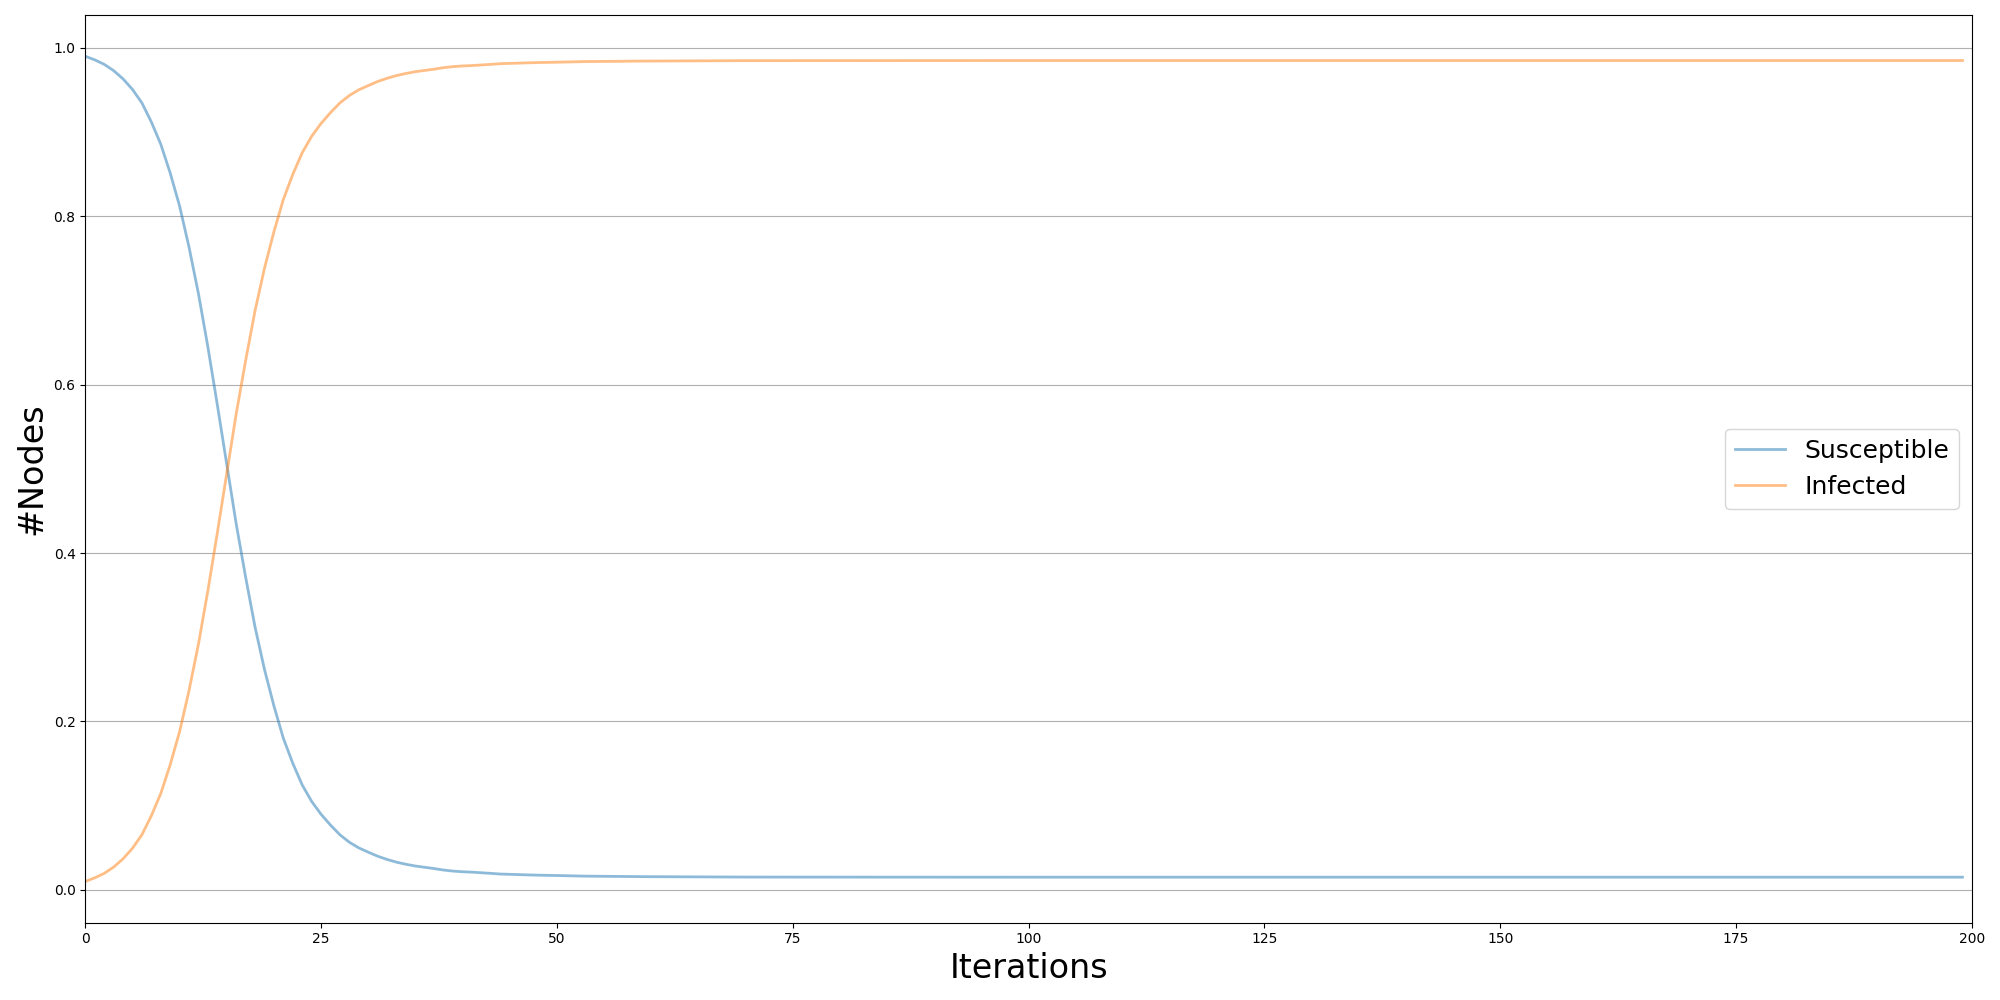
\includegraphics[width=0.45\textwidth]{img/SI/diffusionERSI_beta=0.1_frac=0.01.png}
    \caption{Diffusion trends for the SI model on an Erdos-Renyi graph for $\beta = 0.1$ and initial infected fraction $1\%$}
    \label{fig:my_label}
\end{figure}

\begin{figure}[!htbp]
    \centering
    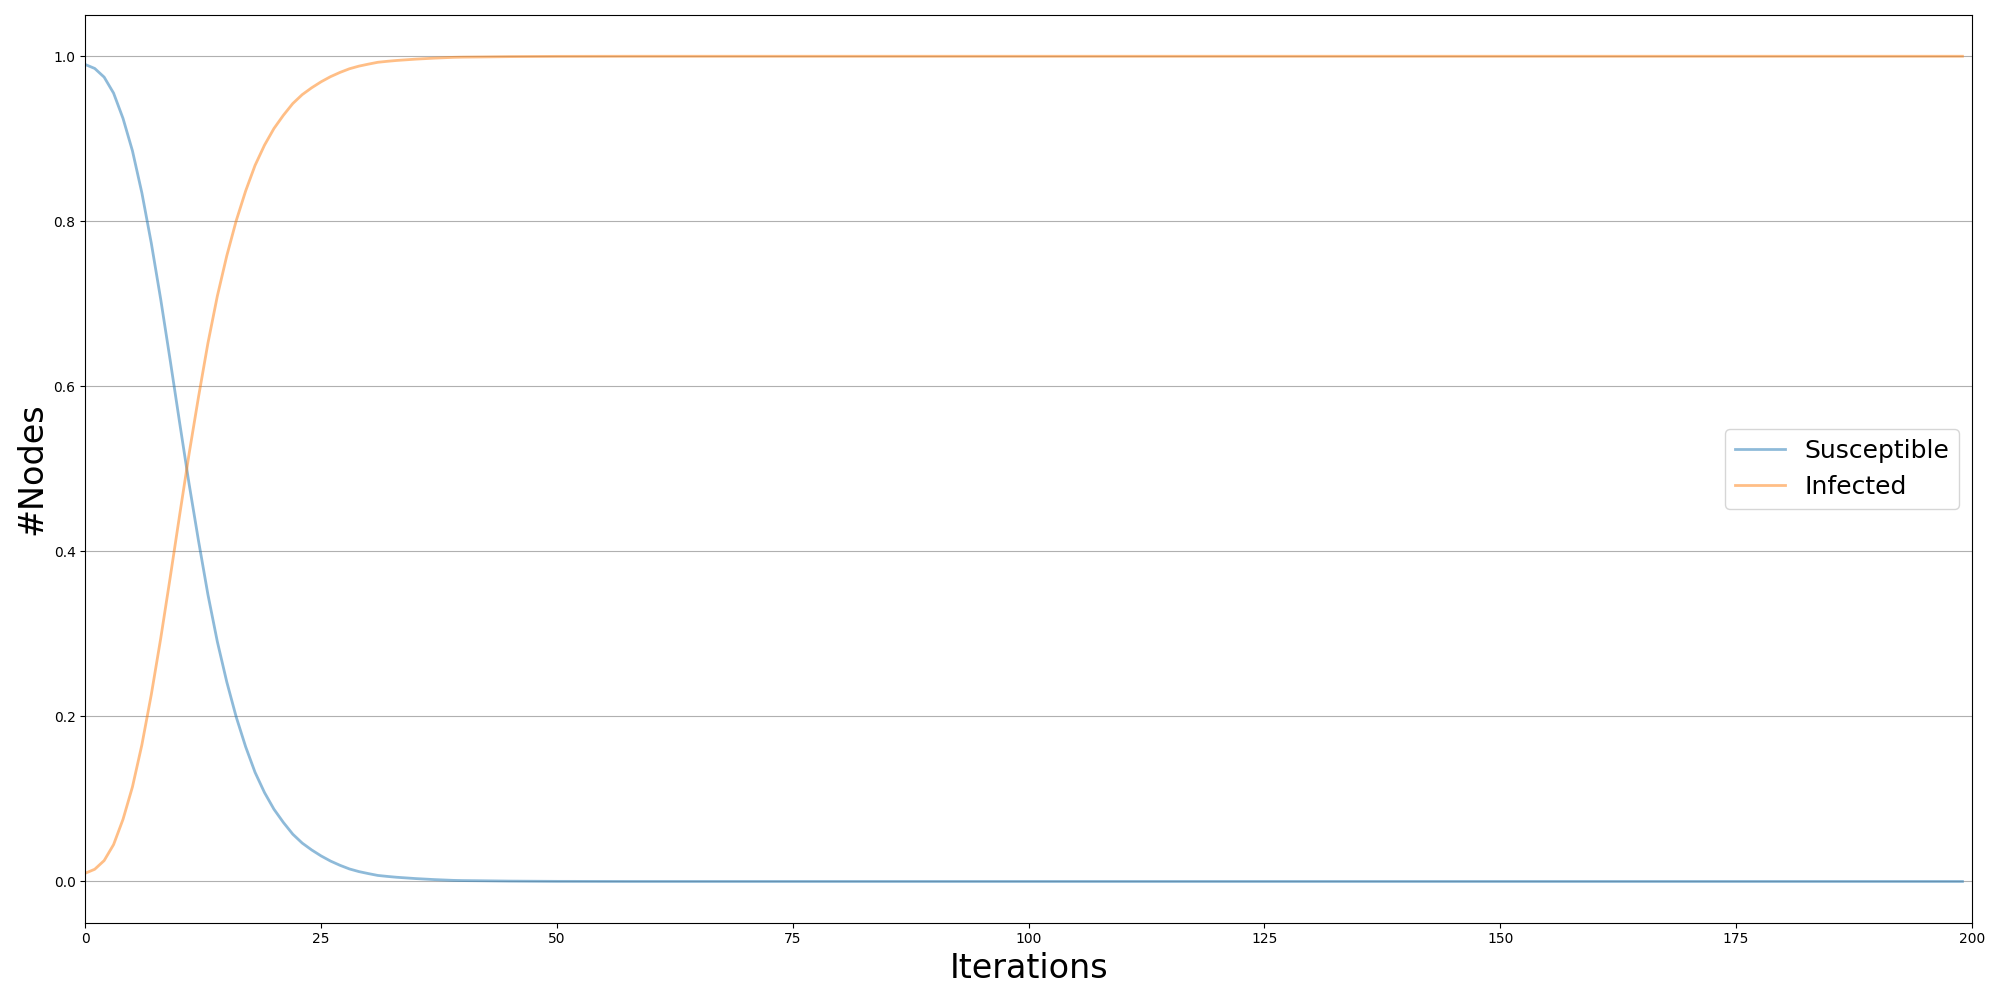
\includegraphics[width=0.45\textwidth]{img/SI/diffusionBASI_beta=0.1_frac=0.01.png}
    \caption{Diffusion trends for the SI model on a Barabasi Albert graph for $\beta = 0.1$ and initial infected fraction $1\%$}
    \label{fig:my_label}
\end{figure}

\begin{figure}[!htbp]
    \centering
    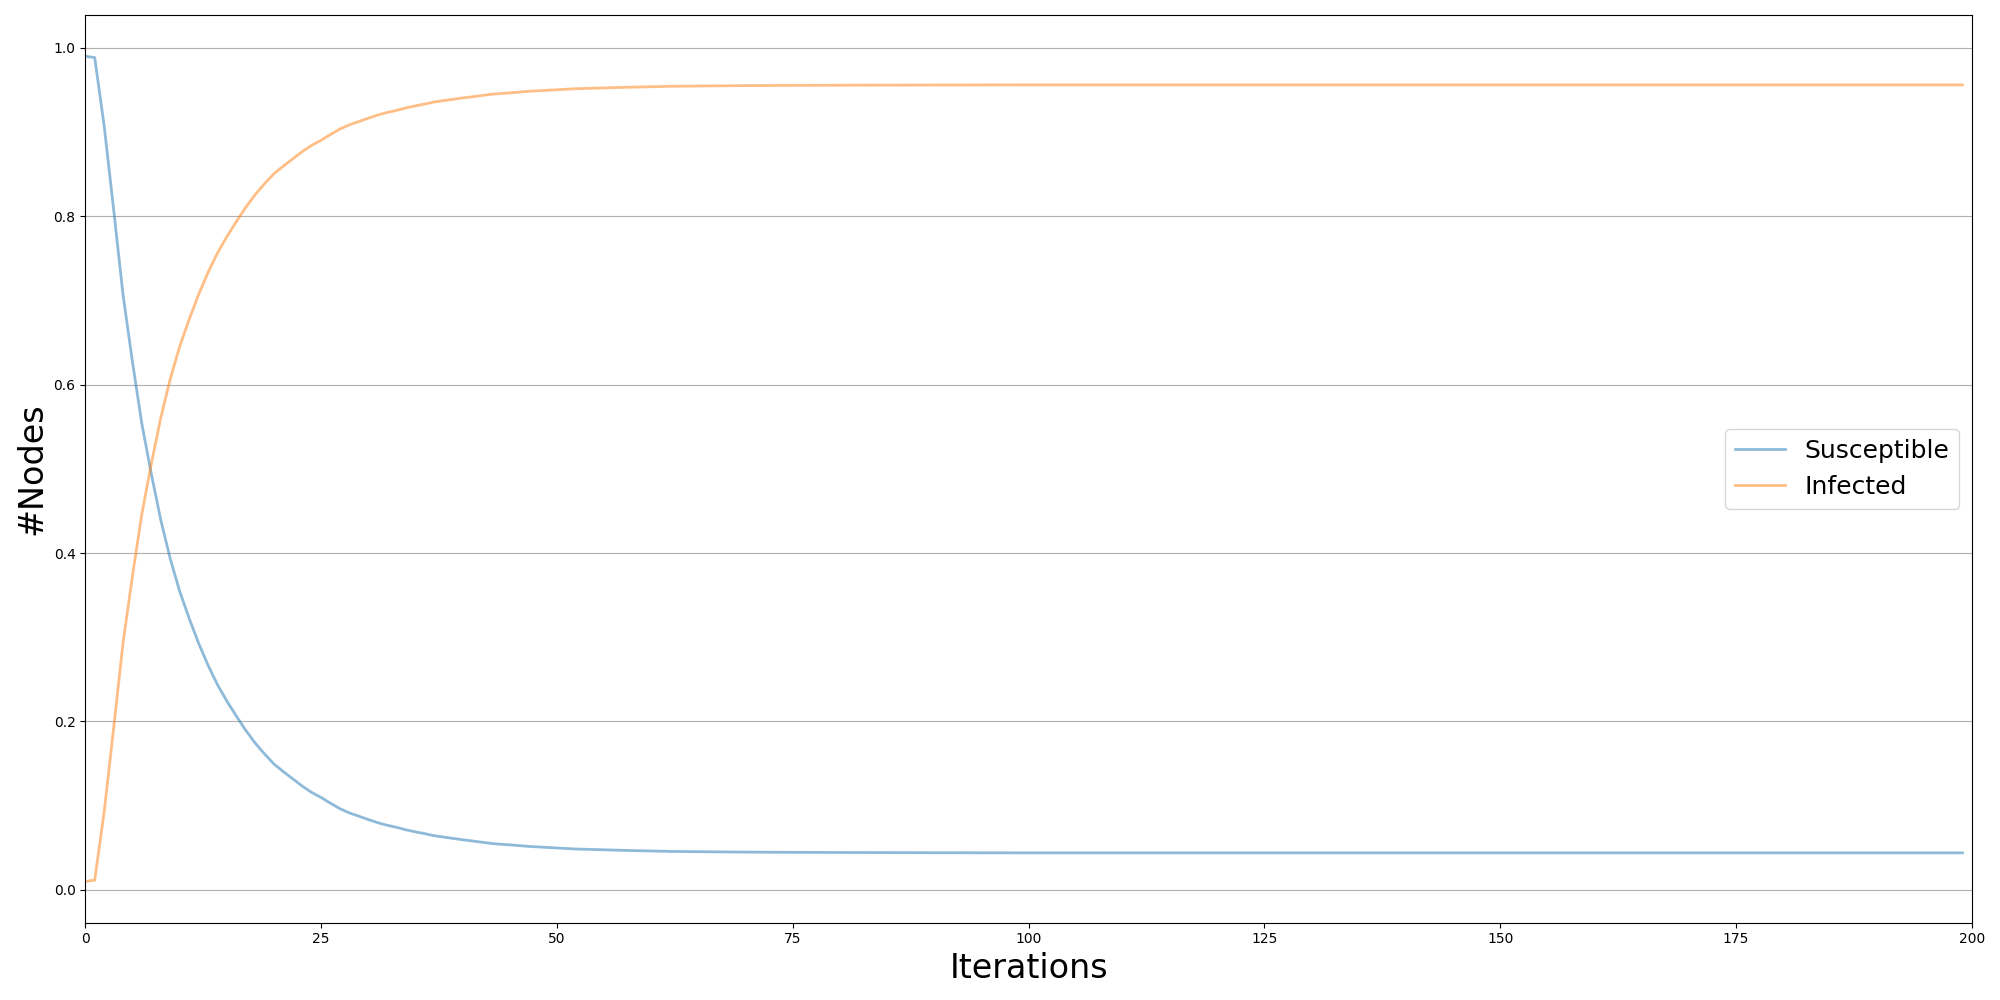
\includegraphics[width=0.45\textwidth]{img/SI/diffusionOurSI_beta=0.1_frac=0.01.png}
    \caption{Diffusion trends for the SI model on our graph for $\beta = 0.1$ and initial infected fraction $1\%$}
    \label{fig:my_label}
\end{figure}
To compare the spread of the "disease" in different network topologies with the SI model we decided to simulate its evolution with different parameters: namely, we simulated $\beta$ from $0.1$ to $1.0$ in incremental steps of $0.1$ and we also varied the initial infection seed from $0.01$ to $0.1$. The results are essentially what was expected: varying either the $\beta$ parameter or the initial infection seed accelerates the spread of the disease (i.e. moves the curves in figure 3,4 and 5 to the left). It is to be noted that both our graph and the ER graph don't reach 1 but slightly lower: this is caused by the fact that these two graphs have more than 1 connected component and if the initial infection seed does not include a member of one of the components the disease has no way of reaching it. Again as expected, the initial "exponential" phase is smaller in our graph (where it is basically non existent) and in the Barabasi Albert graph, where it is visible but small. As stated in the beginning, this is due to the $\gamma$ parameter in the power law distribution, which is $3$ (from theory) in the Barabasi Albert graph and between $2$ and $3$ in our graph.
\subsection{SIS model in different network topologies}
The considerations made for the SI model for the initial exponential phase hold for the SIS model as well. This time, the characteristic time can be written as
$$\tau = \frac{\langle k \rangle}{\beta\langle k^2 \rangle-\mu\langle k \rangle}$$
And, again, we expect that the initial phase is longer in the ER model, slightly shorter in the BA model, and essentially non existent in our graph. This is illustrated in figures 6, 7 and 8. However, other kinds of behaviours emerge. We can clearly see that the fraction of infected nodes is lower in our graph with respect to the ER and BA graph. This can also be traced back to the degree distribution of the graph: in the evolution of the $i$ variable in the SIS model on graphs there is a term $k$ that represents the degree of the node. Most of our nodes have very low degree, while very few have very high degree, so most nodes will have a low probability of being infected. In the Barabasi Albert model this same effect is there, but less pronounced: this is both for the higher $\gamma$ exponent in the degree distribution and the fact that the minimum degree is bounded below by $2$, by construction.

\begin{figure}[!htbp]
    \centering
    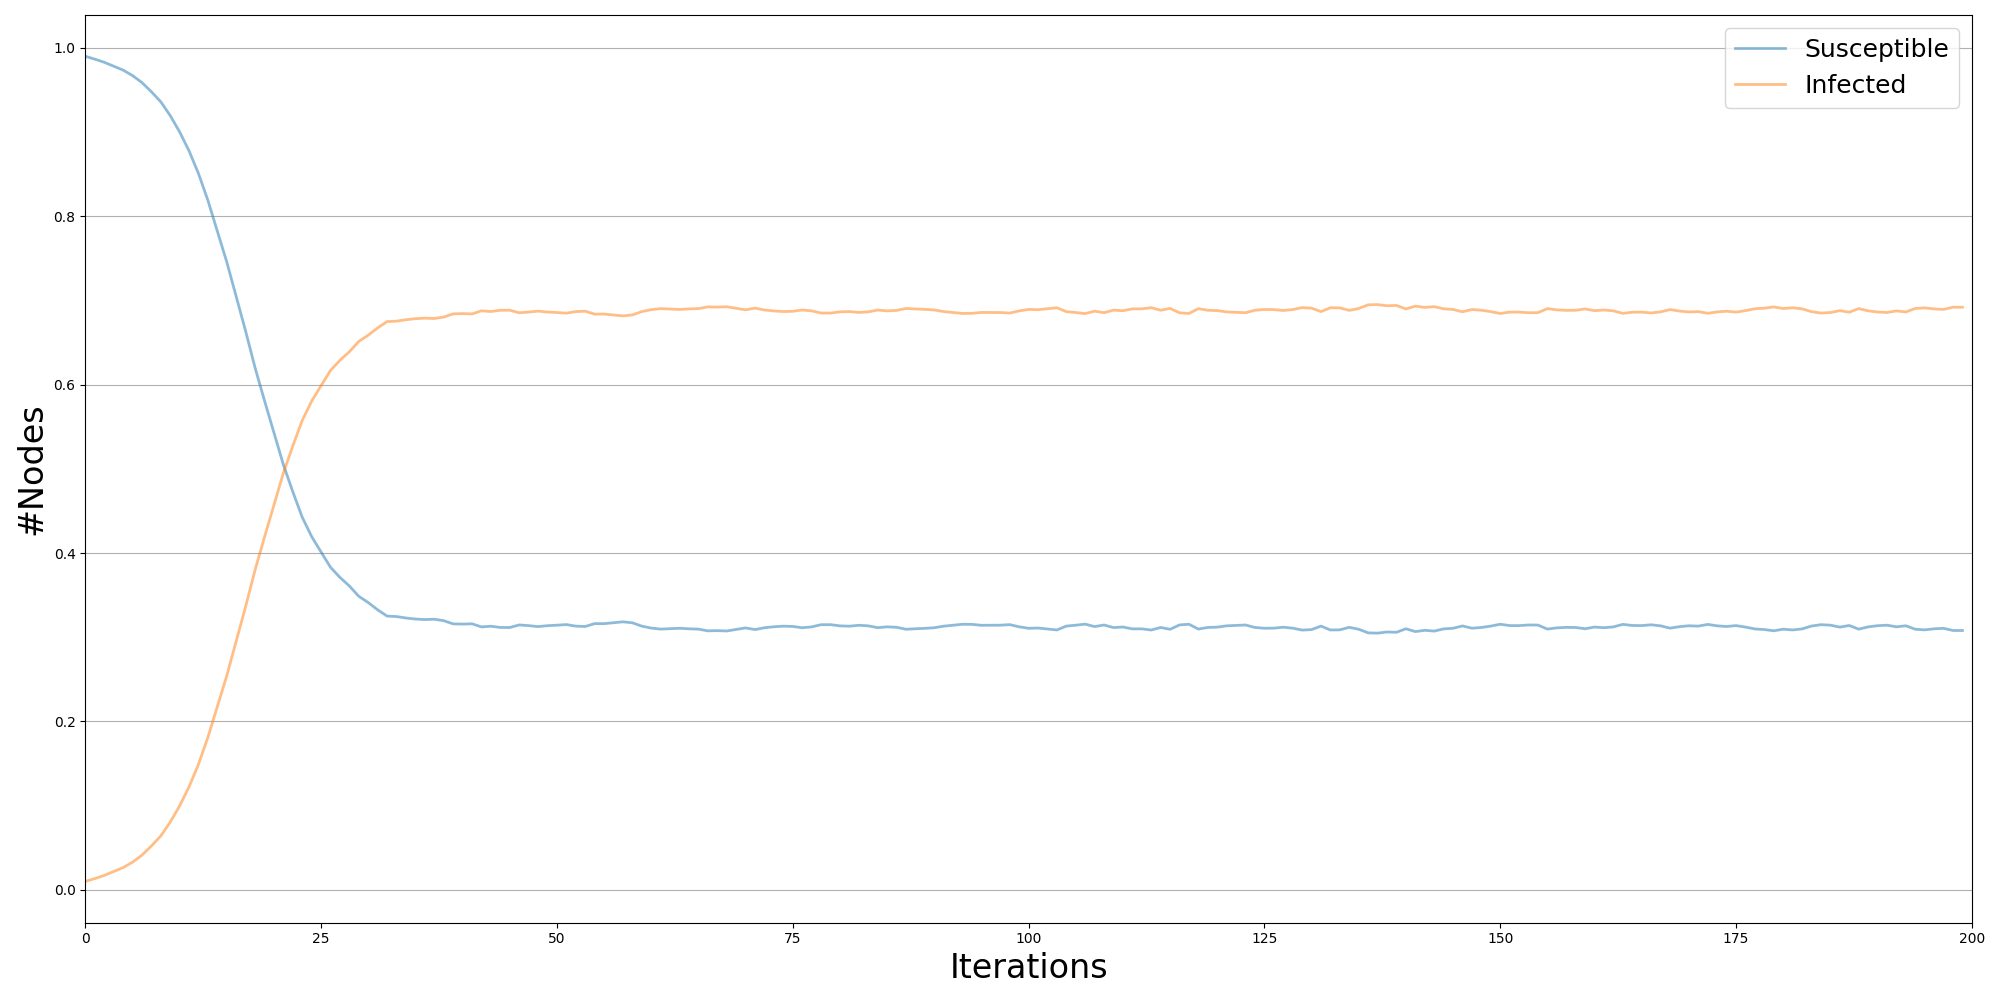
\includegraphics[width=0.45\textwidth]{img/SIS/diffusionERSIS_beta=0.1_mu0.1_frac=0.01.png}
    \caption{Diffusion trends for the SIS model on an Erdos-Renyi graph for $\beta = 0.1$, $\mu = 0.1$ and initial infected fraction $1\%$}
    \label{fig:my_label}
\end{figure}

\begin{figure}[!htbp]
    \centering
    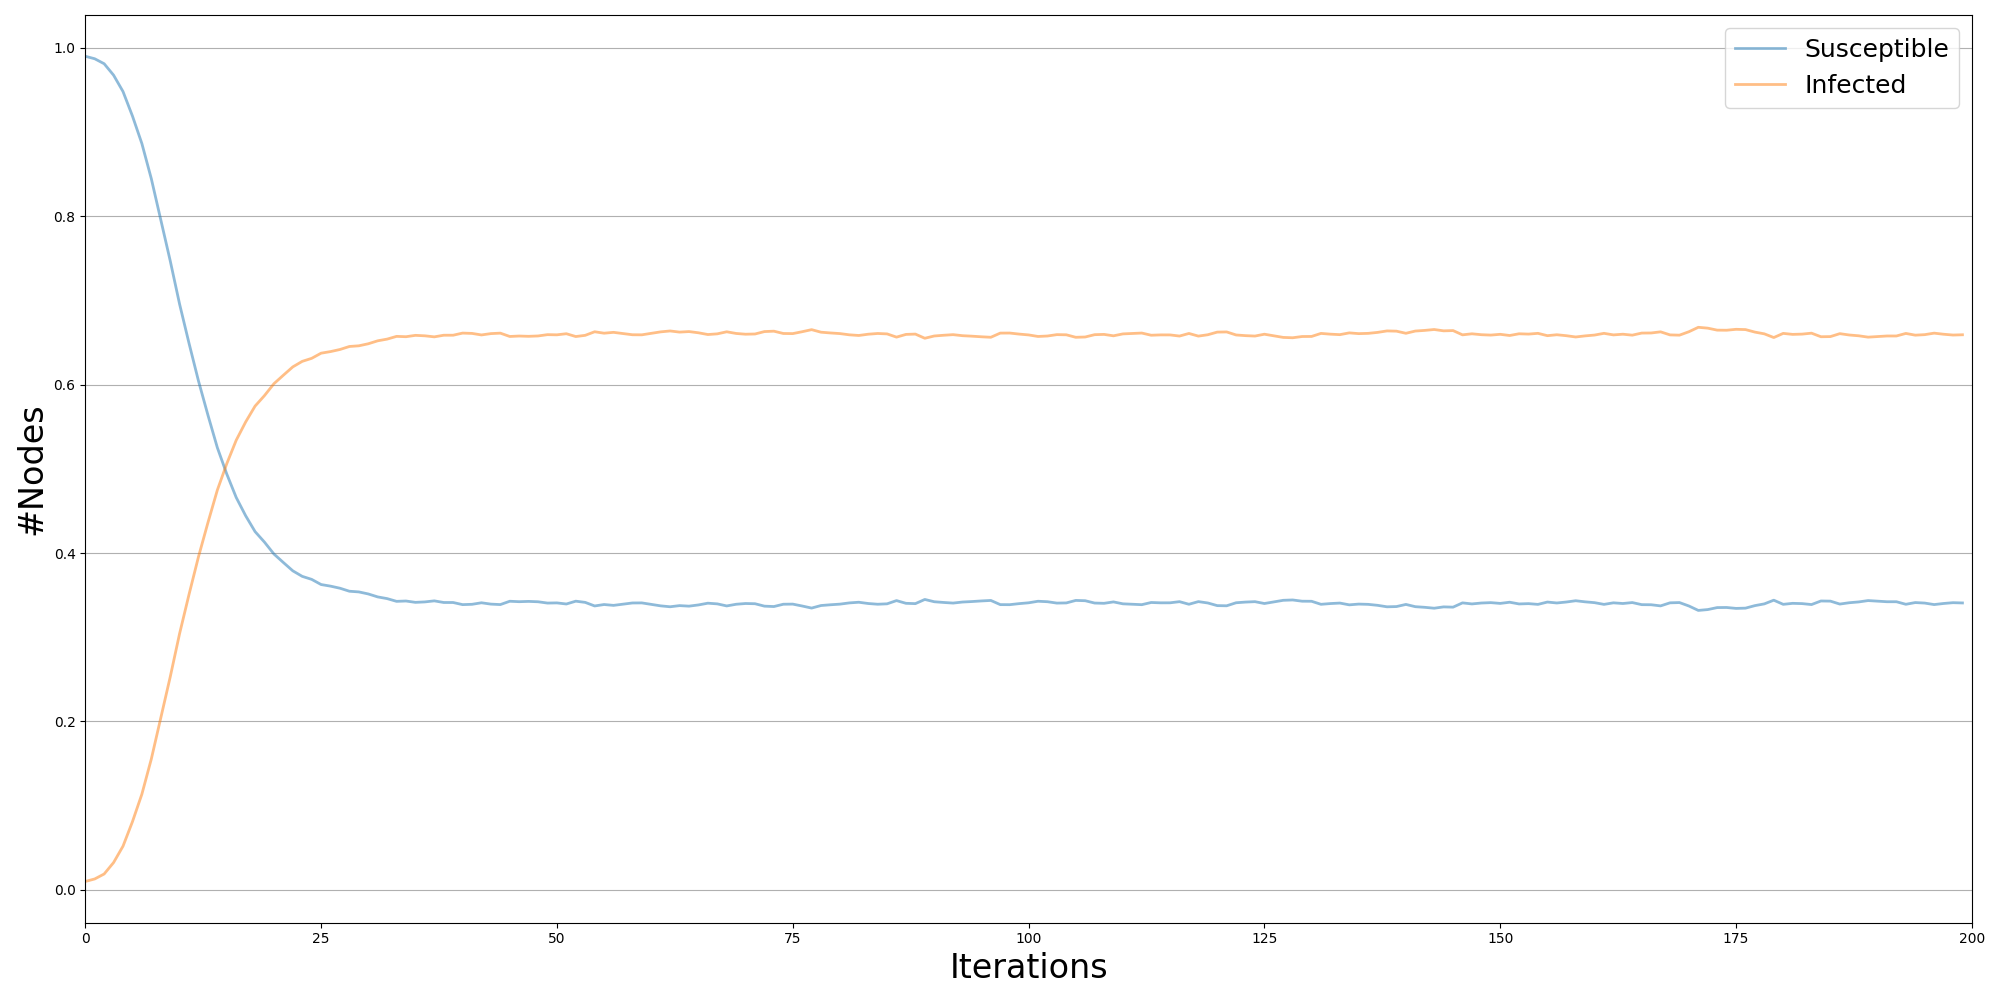
\includegraphics[width=0.45\textwidth]{img/SIS/diffusionBASIS_beta=0.1_mu0.1_frac=0.01.png}
    \caption{Diffusion trends for the SIS model on a Barabasi Albert graph for $\beta = 0.1$, $\mu = 0.1$ and initial infected fraction $1\%$}
    \label{fig:my_label}
\end{figure}

\begin{figure}[!htbp]
    \centering
    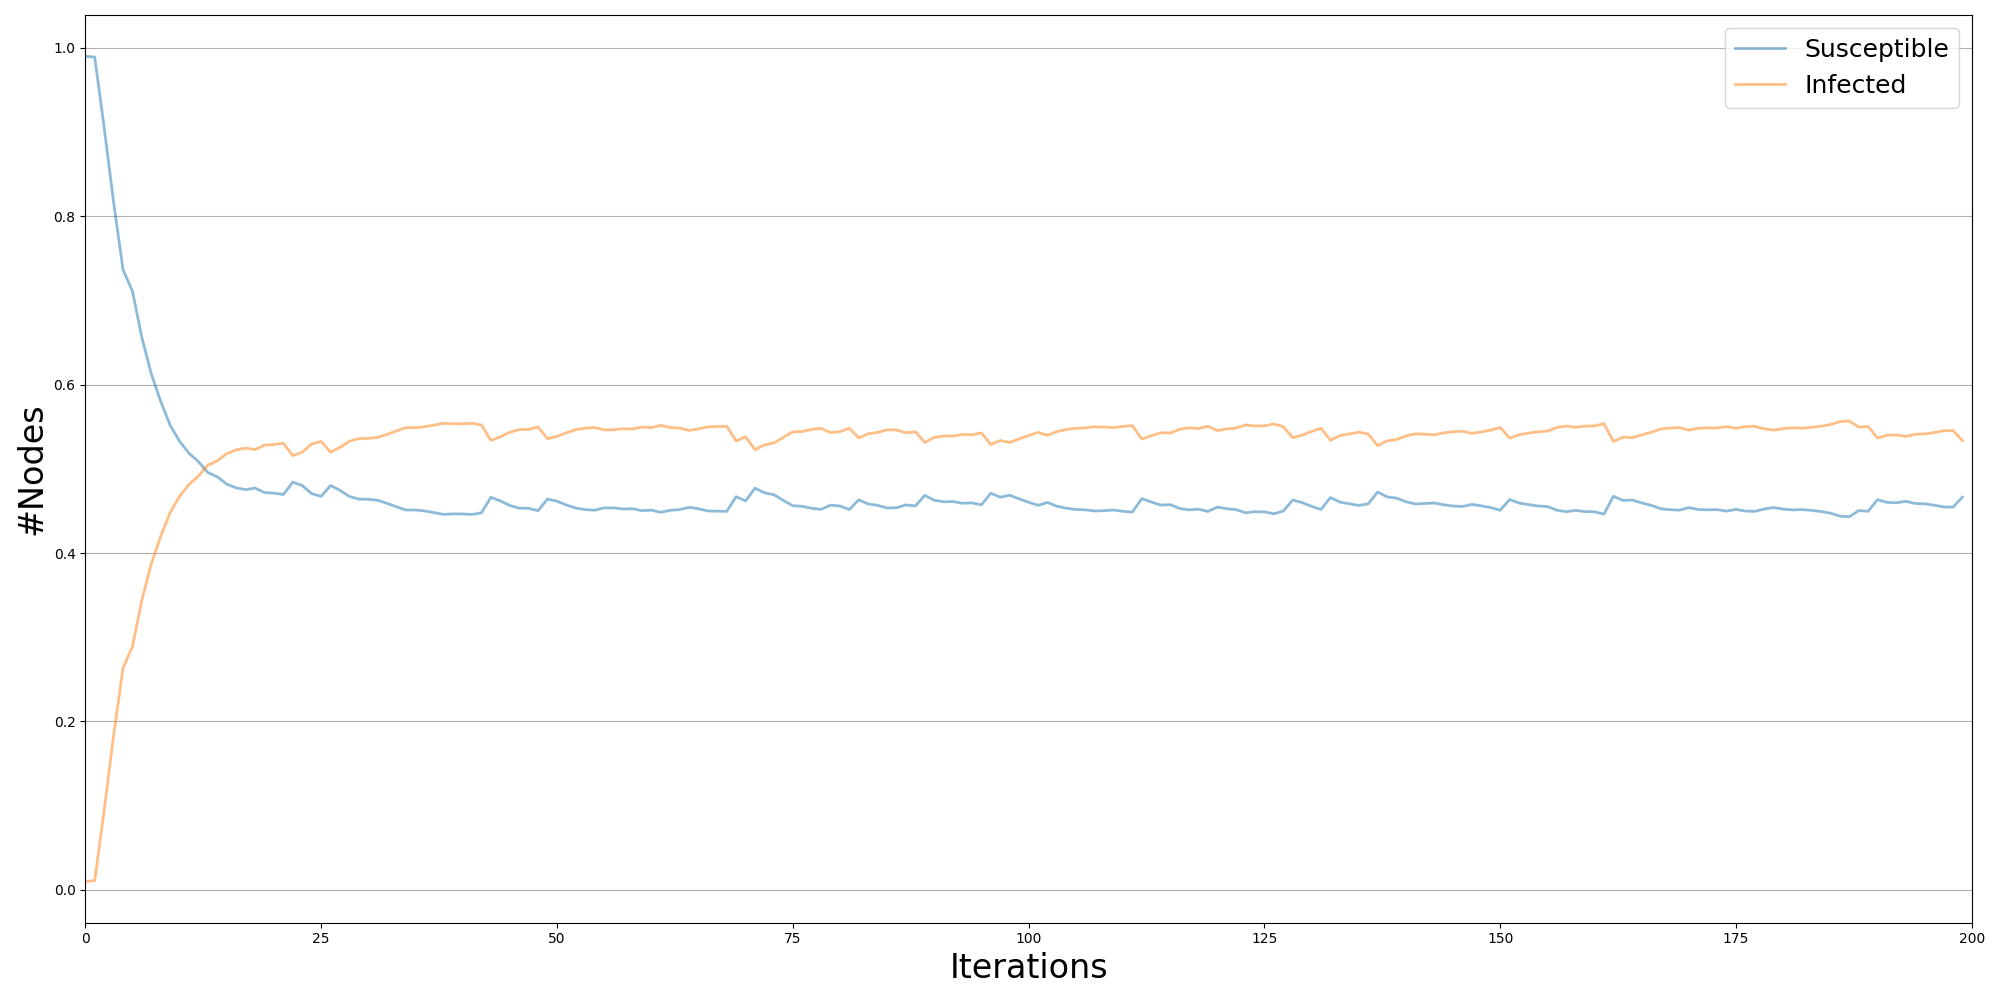
\includegraphics[width=0.45\textwidth]{img/SIS/diffusionOurSIS_beta=0.1_mu0.1_frac=0.01.png}
    \caption{Diffusion trends for the SIS model on our graph for $\beta = 0.1$, $\mu = 0.1$ and initial infected fraction $1\%$}
    \label{fig:my_label}
\end{figure}
There is another behaviour that is of importance that has to be underlined. The persistence of the virus in the population (i.e. if the virus eventually dies down and there are no more infected nodes) is also determined by the node distribution. In an ER graph, if we set $\tau >0$ (that is, an exponential increase), we reach that if $\frac{\beta\langle k \rangle}{\mu} < 1$ the virus does not persist in the population. This is called the \textit{epidemic threshold}. This behaviour can be seen in figure 9.


\begin{figure}[!htbp]
    \centering
    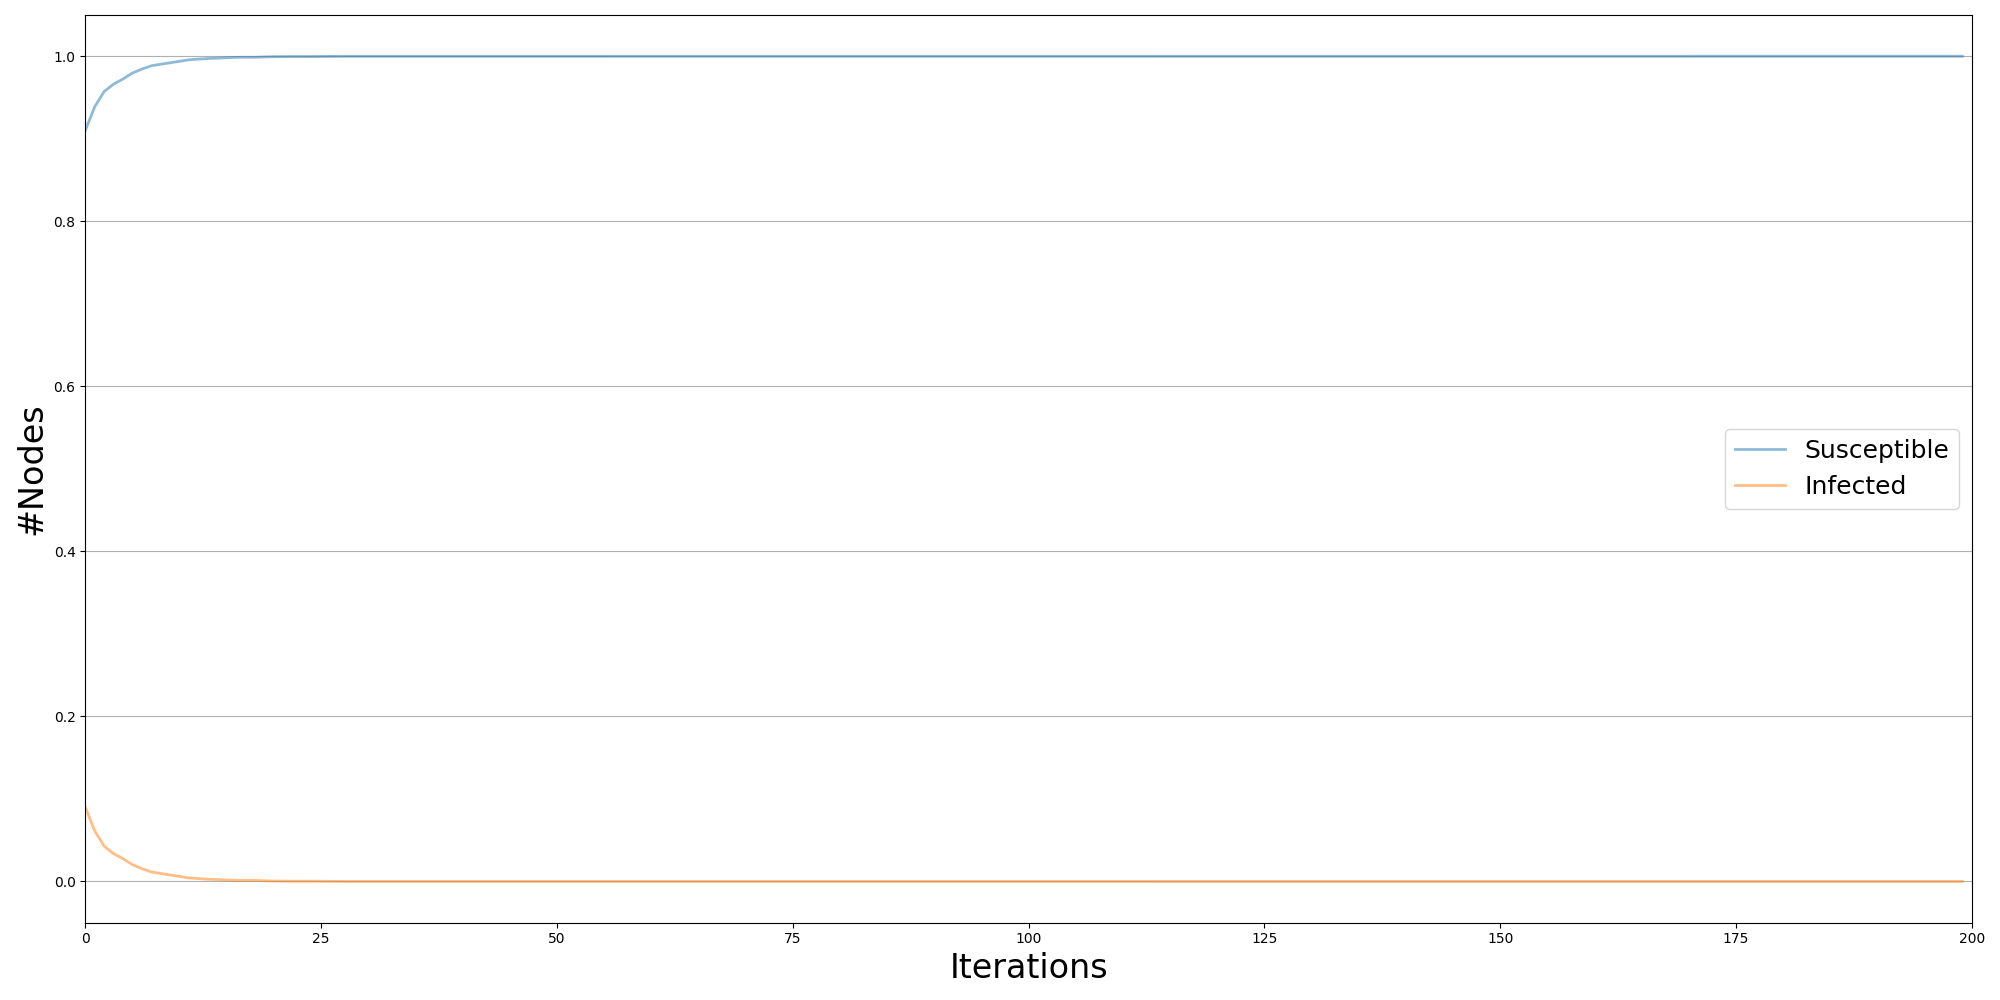
\includegraphics[width=0.45\textwidth]{img/SIS/demonstrationDying.png}
    \caption{Diffusion trends for the SIS model on an ER graph for $\beta = 0.1$, $\mu = 0.7$ and initial infected fraction $9\%$}
    \label{fig:my_label}
\end{figure}
On the other hand, \textbf{there is no epidemic threshold in scale free networks} (with $\gamma \leq 3$). This is because the same procedure we used for the $ER$ graphs would yield $\frac{\langle k \rangle}{\langle k^2 \rangle}$ as an epidemic threshold, which is 0. Therefore, even the least contagious diseases persist in the population. This agrees with our numerical findings.
\subsection{SIR model in different network topologies}
The analysis of the SIR model in the three chosen topologies is a fairly straightforward extension of the analysis for the SI and SIS models. While the model adds a new compartment and thus is more complex in this regard, most of the considerations made for the previous models hold for the SIR model as well. The characteristic time is
$$\tau = \frac{\langle k \rangle}{\beta\langle k^2 \rangle-(\mu+\beta)\langle k \rangle}$$

\begin{figure}[!htbp]
    \centering
    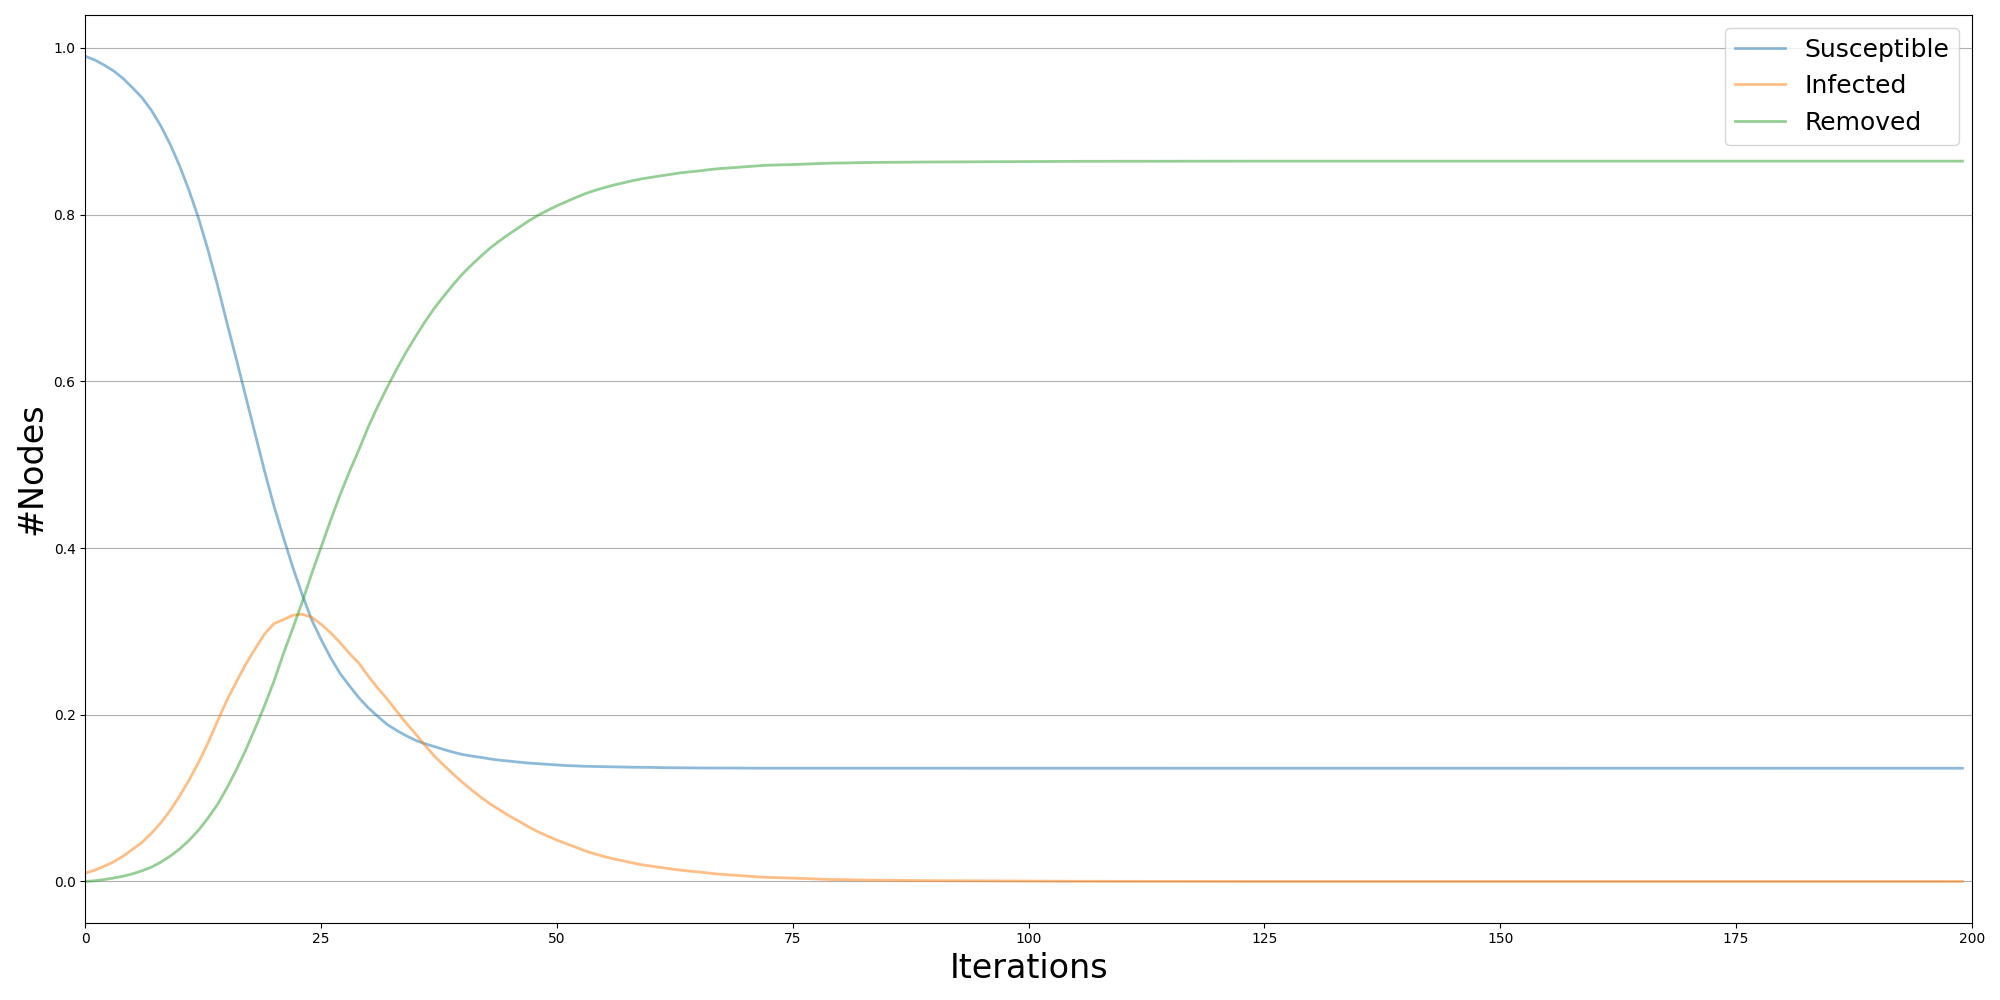
\includegraphics[width=0.45\textwidth]{img/SIR/diffusionERSIR_beta=0.1_mu0.1_frac=0.01.png}
    \caption{Diffusion trends for the SIR model on an Erdos-Renyi graph for $\beta = 0.1$, $\mu = 0.1$ and initial infected fraction $1\%$}
    \label{fig:my_label}
\end{figure}

\begin{figure}[!htbp]
    \centering
    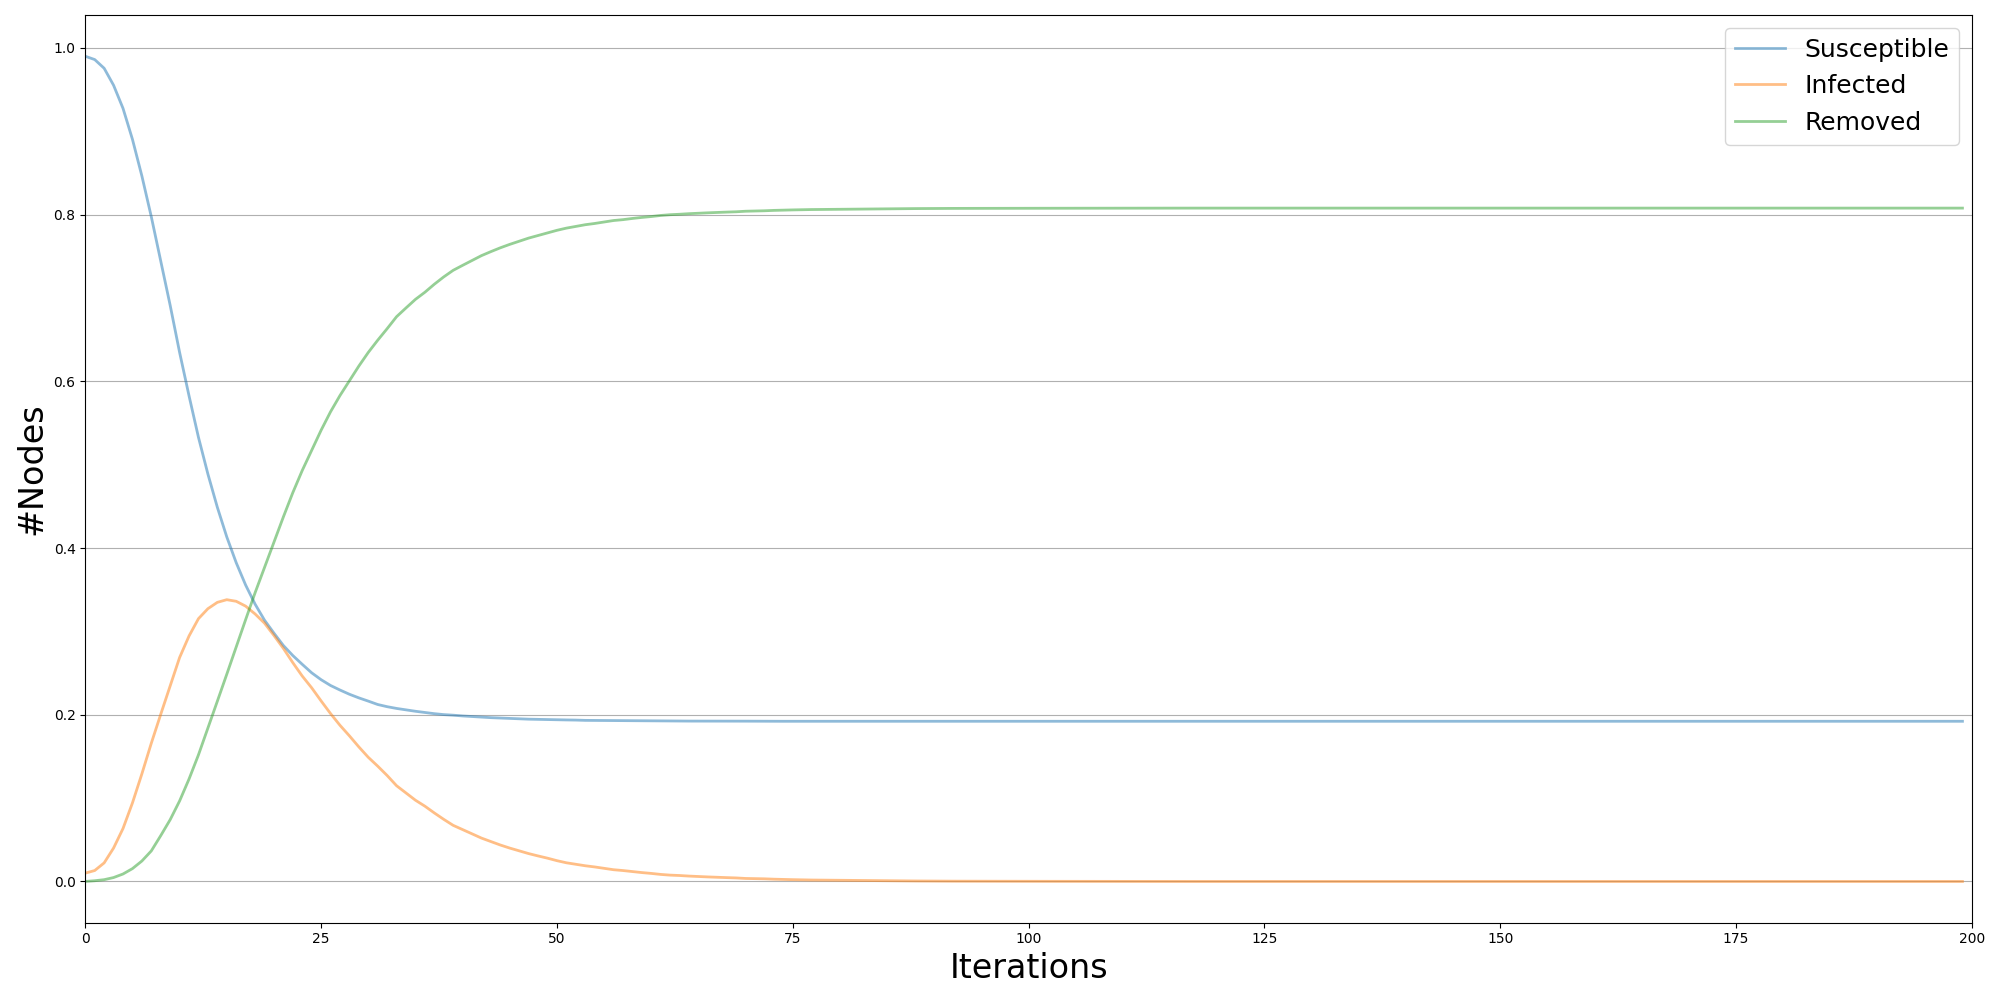
\includegraphics[width=0.45\textwidth]{img/SIR/diffusionBASIR_beta=0.1_mu0.1_frac=0.01.png}
    \caption{Diffusion trends for the SIR model on a Barabasi Albert graph for $\beta = 0.1$, $\mu = 0.1$ and initial infected fraction $1\%$}
    \label{fig:my_label}
\end{figure}
\begin{figure}[!htbp]
    \centering
    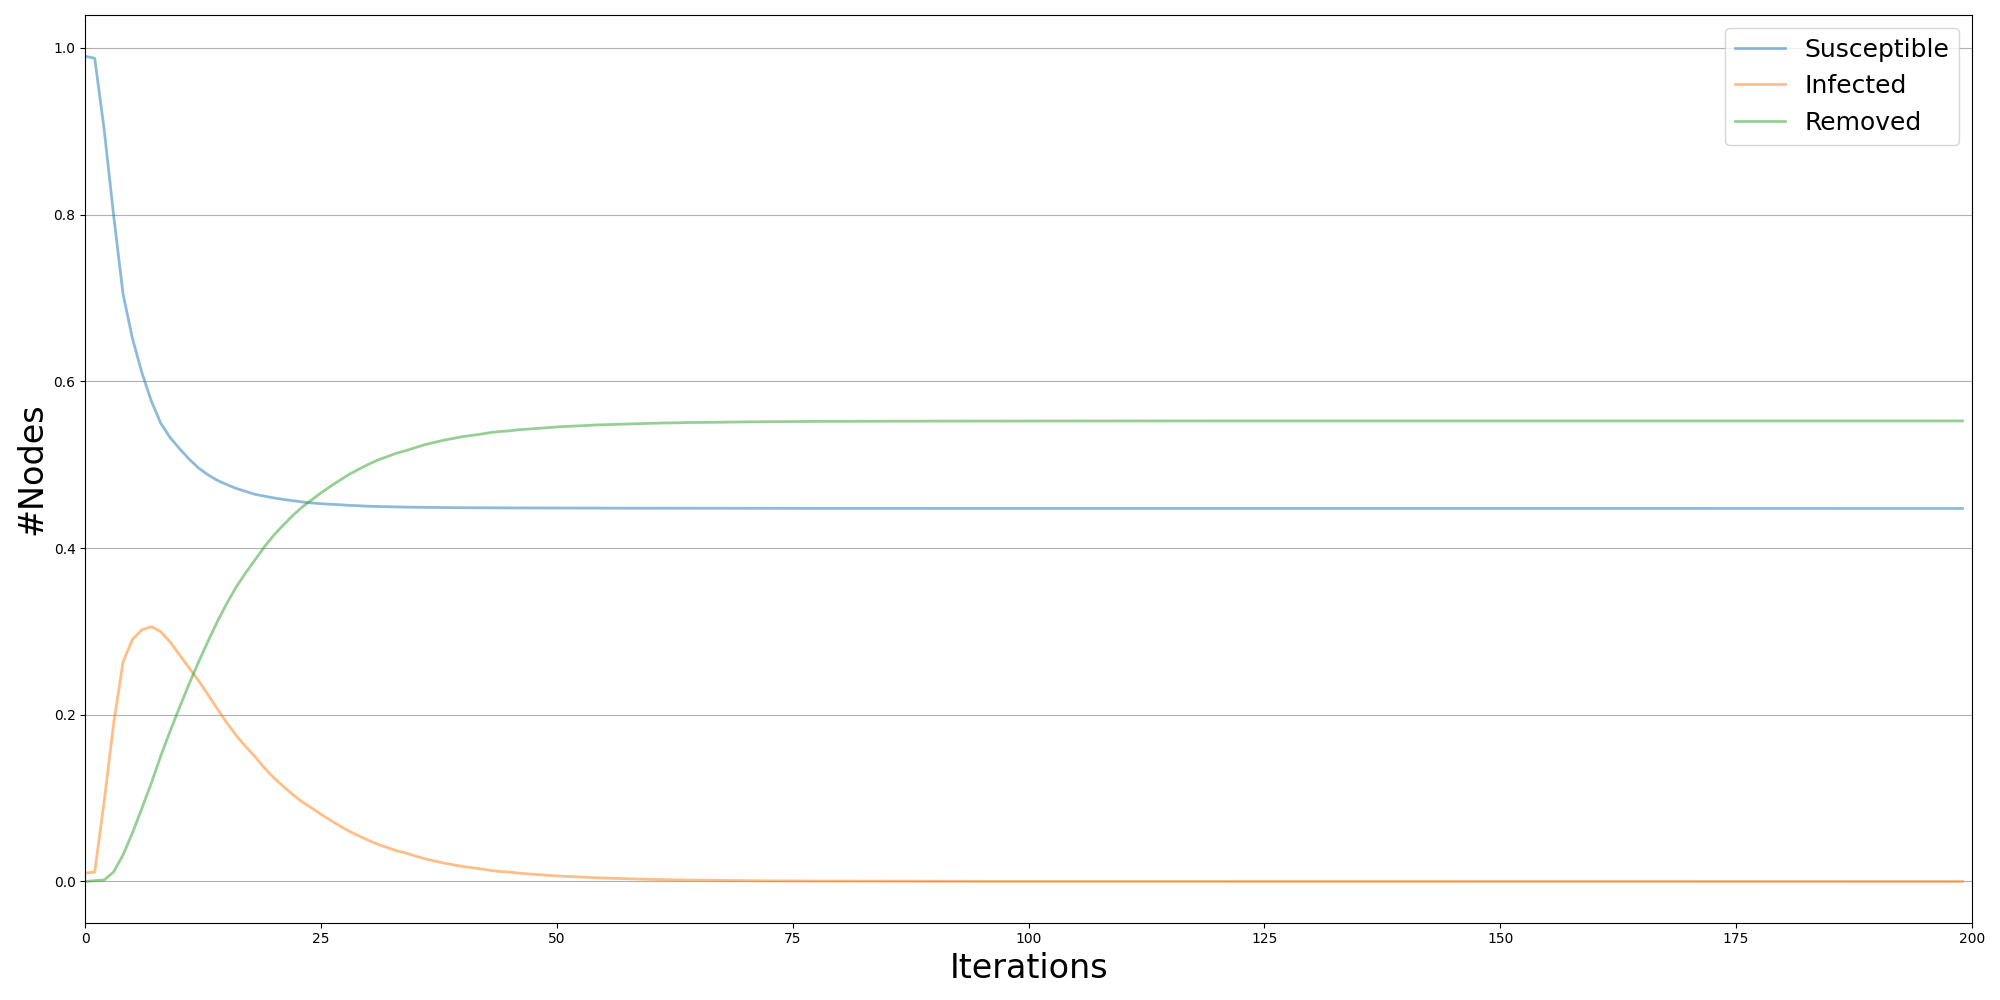
\includegraphics[width=0.45\textwidth]{img/SIR/diffusionOurSIR_beta=0.1_mu0.1_frac=0.01.png}
    \caption{Diffusion trends for the SIR model on our graph for $\beta = 0.1$, $\mu = 0.1$ and initial infected fraction $1\%$}
    \label{fig:my_label}
\end{figure}
As expected, the exponential phase the longest in the ER graph, shorter in the BA graph and essentially non existent in our graph (as can be seen in figures 10, 11 and 12). Again, the epidemic threshold is $0$ in both the Barabasi Albert graph and our graph, while being finite in the ER graph $$\lambda_c = \frac{1}{\frac{\langle k^2 \rangle}{\langle k \rangle}-1}$$
Behaviour with $\frac{\beta}{\mu} < \lambda_c$ is demonstrated in figure 13.


\begin{figure}[!htbp]
    \centering
    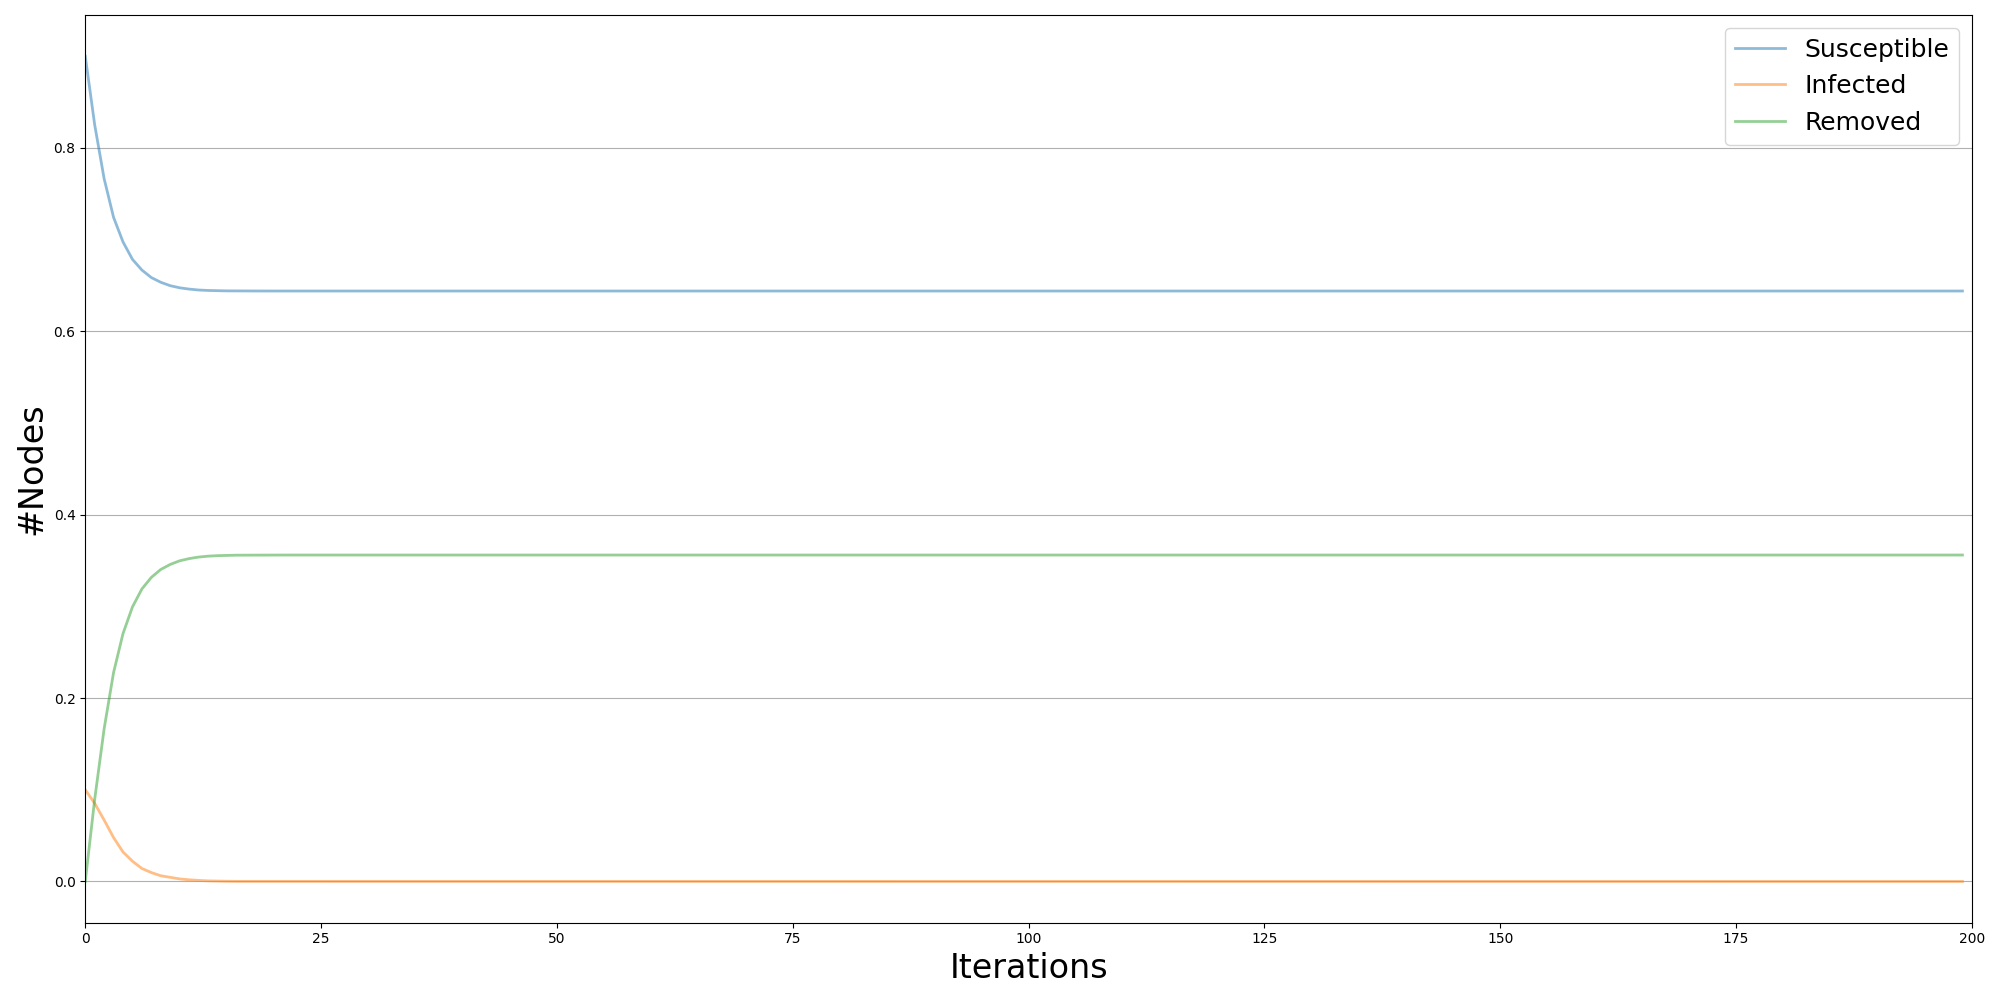
\includegraphics[width=0.45\textwidth]{img/SIR/dyingDemonstration.png}
    \caption{Demonstration for parameters below the epidemic threshold for the SIR model on our graph for $\beta = 0.2$, $\mu = 0.9$ and initial infected fraction $10\%$}
    \label{fig:my_label}
\end{figure}

\subsection{Threshold model in different network topologies}
We decided to simulate the model with an initial percentage of infected nodes $1\%$. To choose the thresholds for each node, we have drawn random numbers from a normal distribution with mean $\mu = 0.5$ and $\sigma$ varying from $0.1$ to $5$. Since the threshold is a percentage, if a given drawn threshold turned out to be $<0$ ($>1$) we have given it the value $0$ ($1$). The behaviours turn out to be similar between the three graphs, the number of infected being slightly higher in the BA graph (likely due to the fact that there is only one connected component) and roughly equal in our graph and in the ER graph.

\begin{figure}[!htbp]
    \centering
    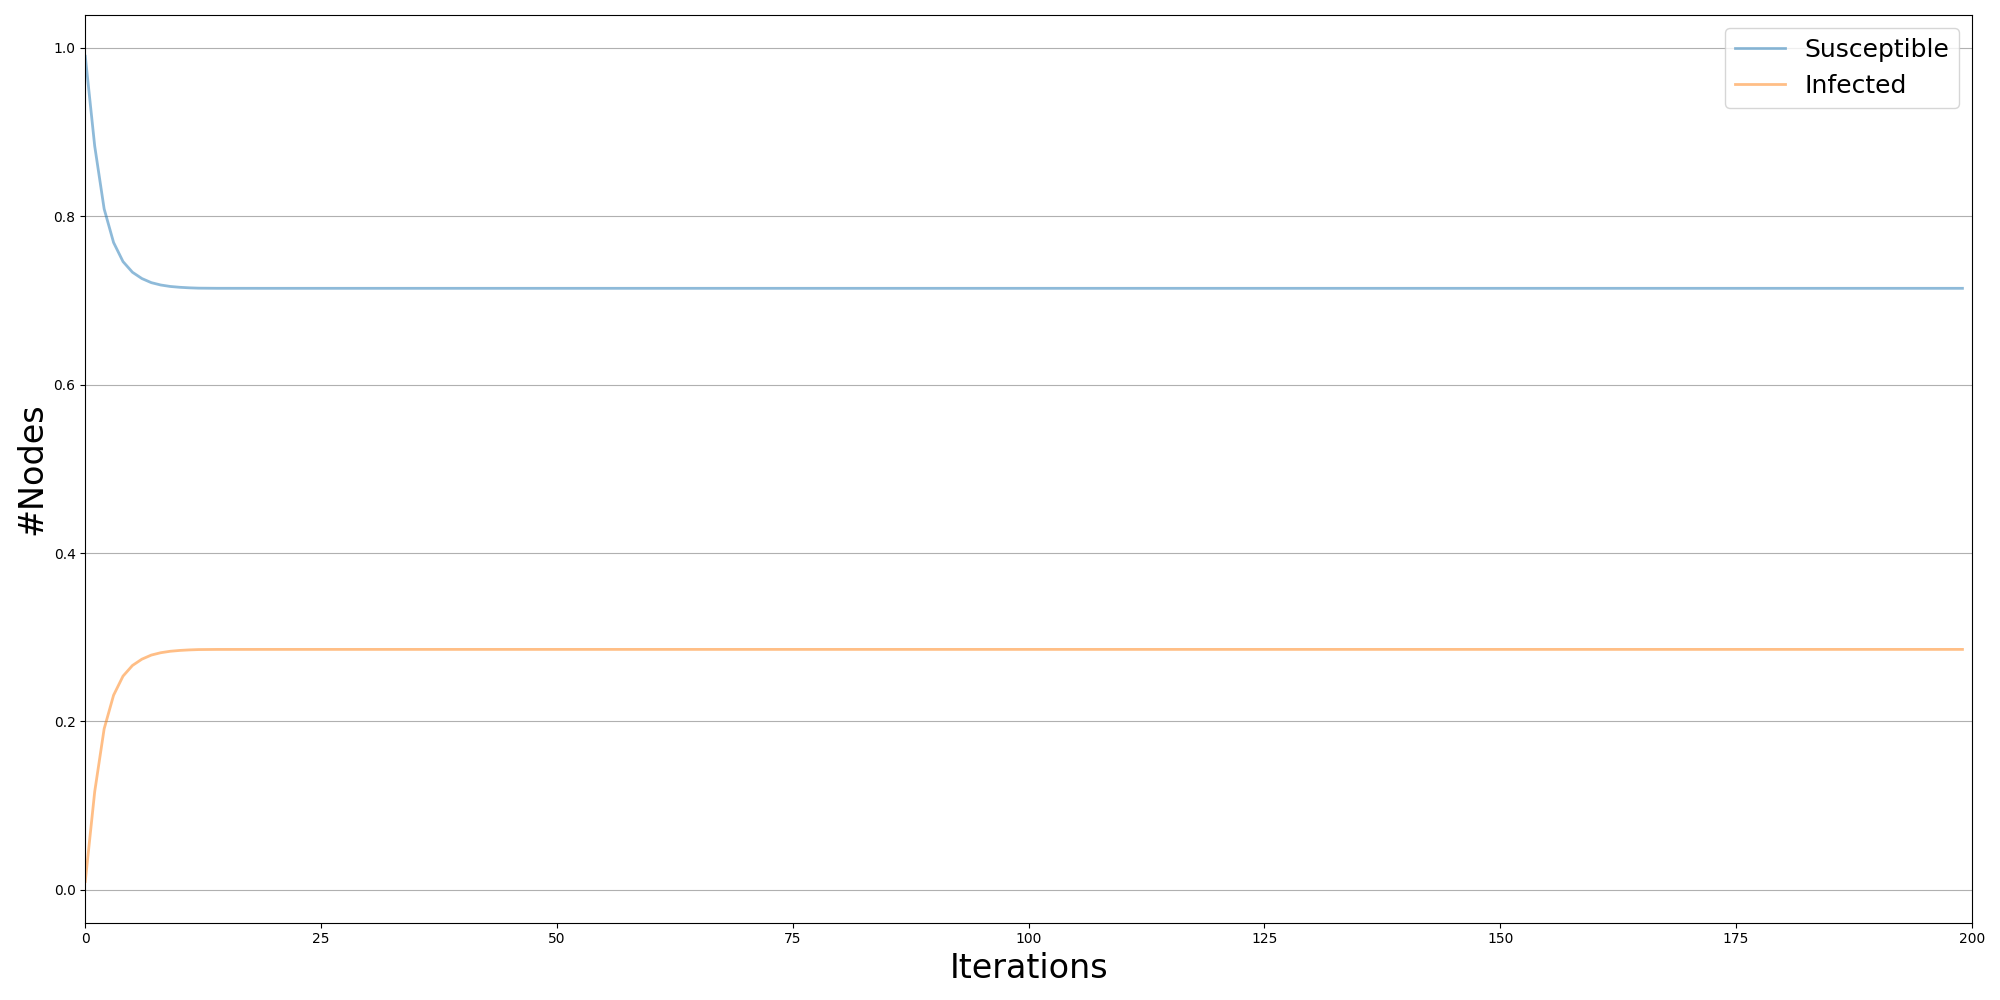
\includegraphics[width=0.45\textwidth]{img/Threshold/diffusionERThreshold_fraction=0.01_mu0.5_sigma=0.4.png}
    \caption{Diffusion trends for the Threshold model on an Erdos-Renyi graph for $\mu = 0.5$, $\sigma = 0.4$ and initial infected fraction $1\%$}
    \label{fig:my_label}
\end{figure}

\begin{figure}[!htbp]
    \centering
    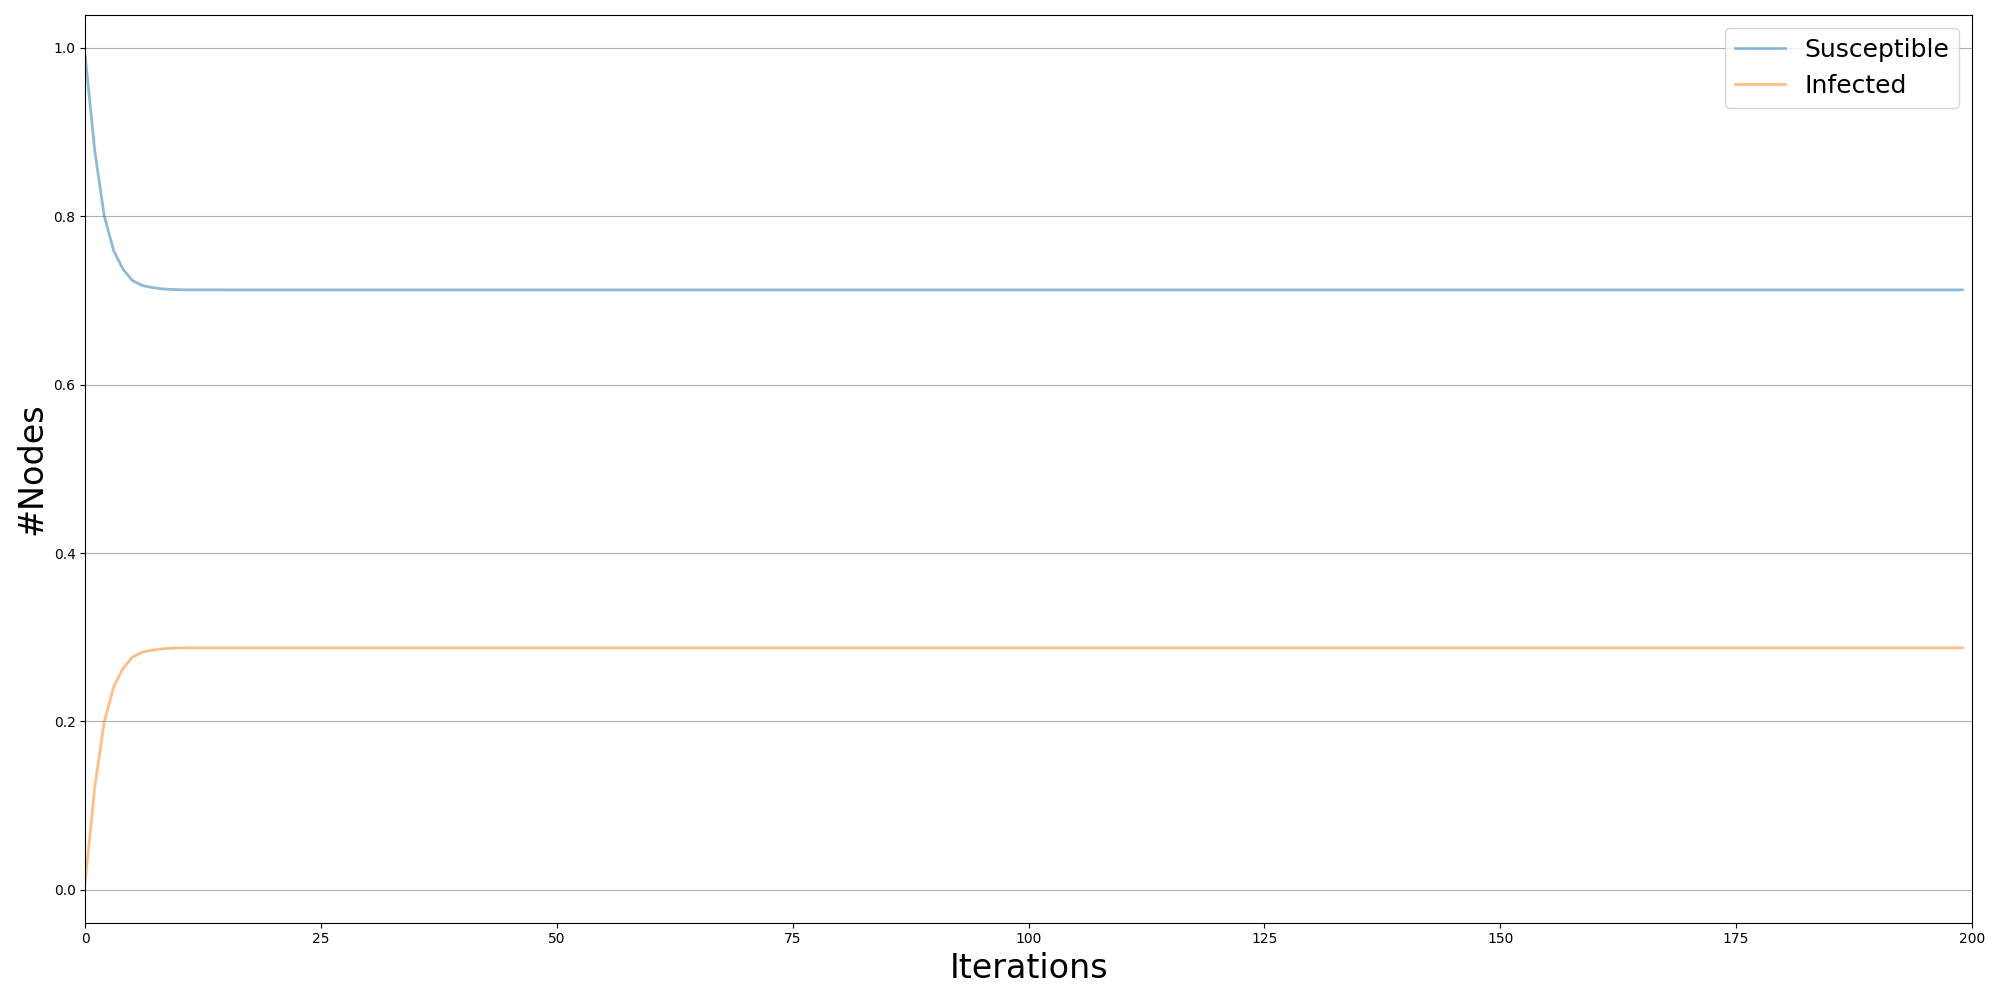
\includegraphics[width=0.45\textwidth]{img/Threshold/diffusionBAThreshold_fraction=0.01_mu0.5_sigma=0.4.png}
    \caption{Diffusion trends for the Threshold model on a Barabasi Albert graph for $\mu = 0.5$, $\sigma = 0.4$ and initial infected fraction $1\%$}
    \label{fig:my_label}
\end{figure}
\begin{figure}[!htbp]
    \centering
    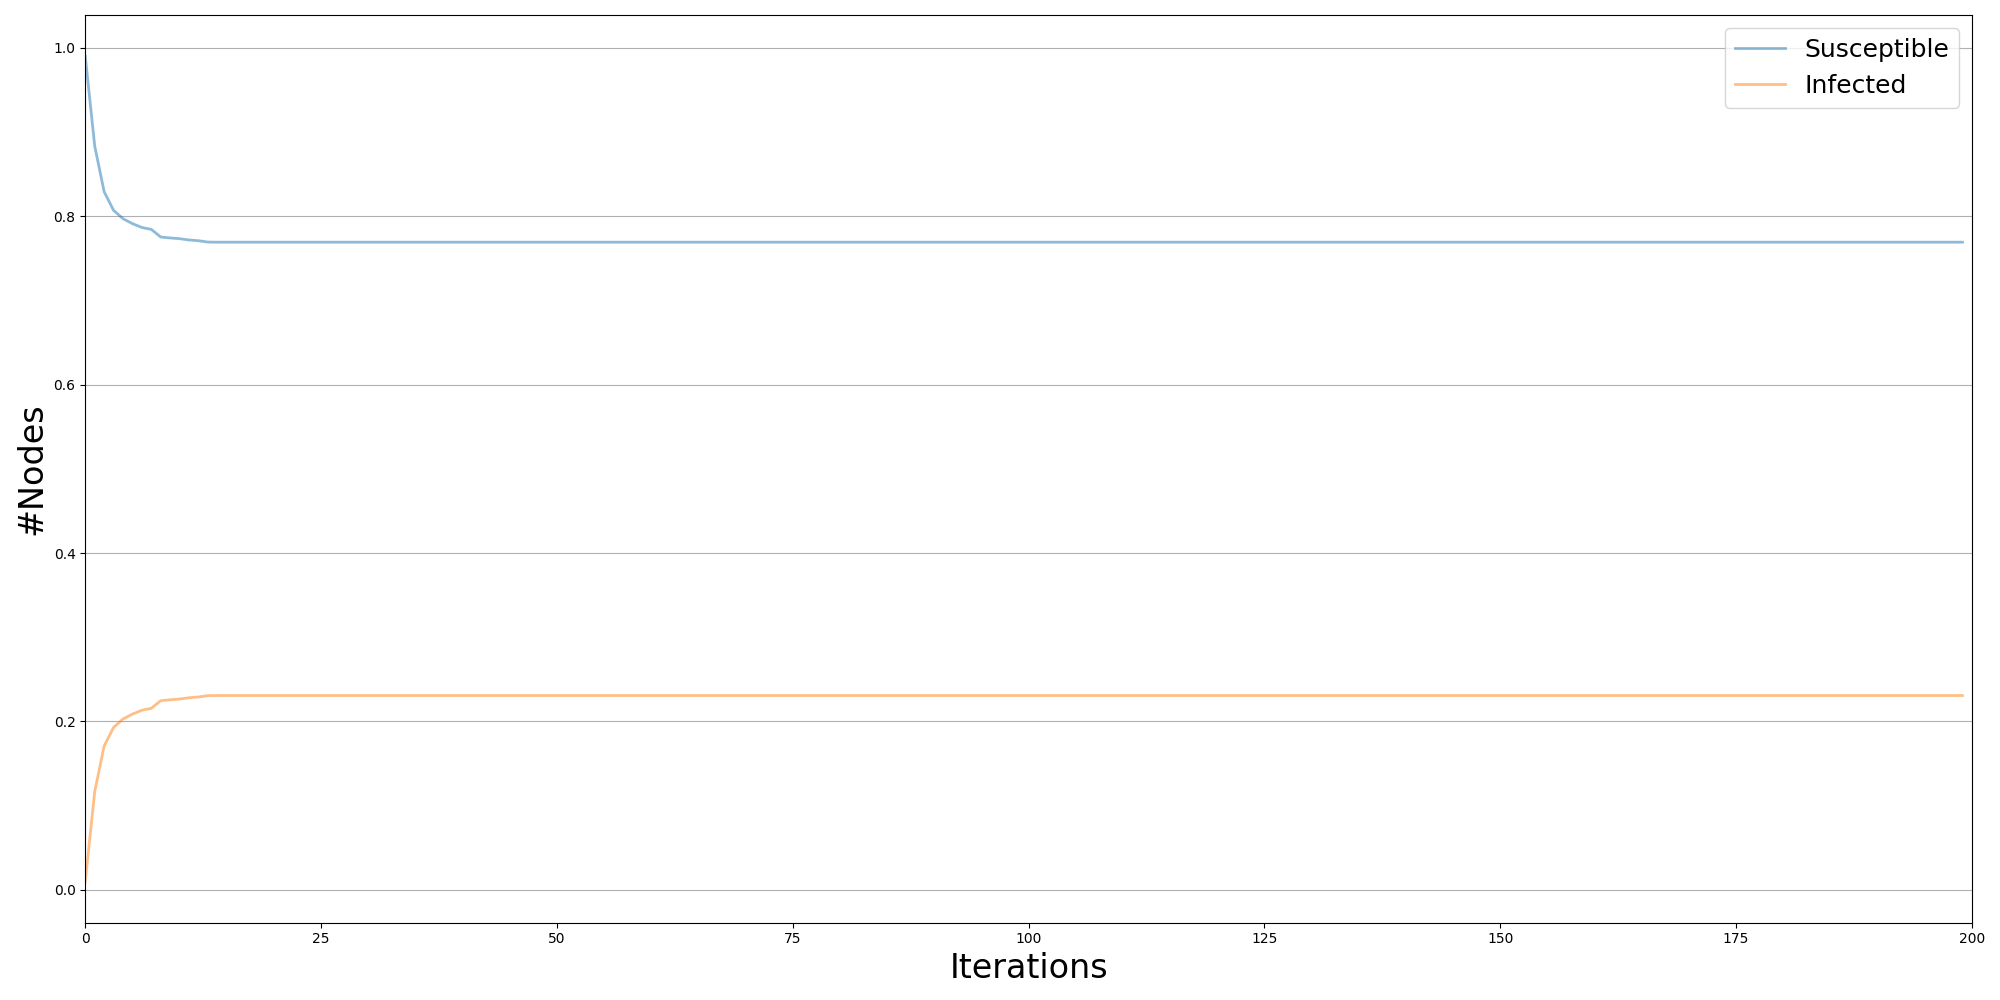
\includegraphics[width=0.45\textwidth]{img/Threshold/diffusionOurThreshold_fraction=0.01_mu0.5_sigma=0.4.png}
    \caption{Diffusion trends for the Threshold model on our graph for $\mu = 0.5$, $\sigma = 0.4$ and initial infected fraction $1\%$}
    \label{fig:my_label}
\end{figure}
If we start from an initial percentage of infected nodes $r(0) = r_0$, on a complete graph, at time $t$ the infected percentage is going to be $F^t(r_0)$, with $F$ as defined earlier and where $F^t$ denotes the composition of $F$ with itself $t$ times. The striking behaviour that emerges from both our analysis and from the original paper is that, initially, increasing $\sigma$ has the effect of increasing the percentage of infected nodes, while increasing $\sigma$ after a certain threshold $\sigma_c$ has the effect of lowering the final percentage of infected nodes.
\begin{figure}[!htbp]
    \centering
    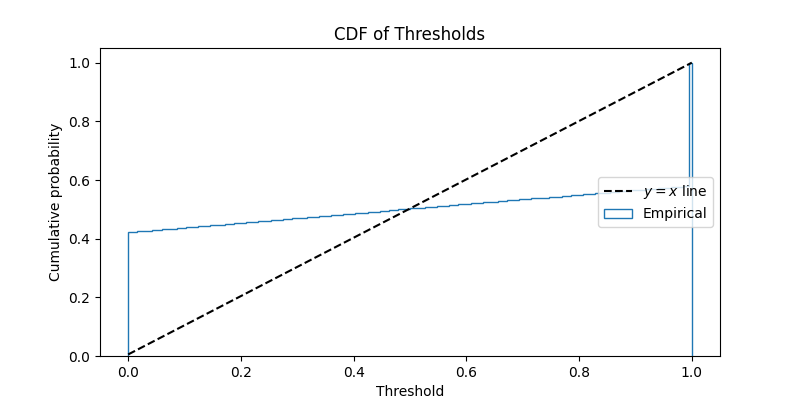
\includegraphics[width=0.45\textwidth]{img/Threshold/demonstrationParallel.png}
    \caption{Cumulative distribution function of a cut normal distribution with $\mu = 0.5$ and $\sigma = 2.5$}
    \label{fig:my_label}
\end{figure}
As we increase sigma after $\sigma_c$ the CDF becomes more and more parallel to the $x$ axis, and the intersection with the $y = x$ line lowers (an example in figure 17). This is due to the fact that we are effectively cutting a distribution that has support on the whole real line to force it between $0$ and $1$: this is also the cause of the artifacts at the edge of the plot.

\section{Task 3: Unsupervised link prediction}
Link prediction is a very relevant topic in network analysis; we might think, as an example, of predictions of friendships on Facebook or Linkedin to suggest friends to the user. In our case what we are trying to predict are future mentions between the users in our graph. To do this, we sampled around 15\% of the nodes in the original network (for computational reasons) and we split the subnetwork in two: about 80\% for training our model, and the remaining 20\% for testing. The split was done temporally, in such a way that we are trying to predict links which will appear in the future. We decided to use an unsupervised approach, i.e. using a set of proximity measures to try to predict which links are going to appear. The algorithms we used are four:
\begin{itemize}
    \item The Common Neighbours algorithm
    \item The Adamic Adar algorithm
    \item The Jaccard algorithm
    \item The Preferential attachment algorithm
\end{itemize}
A brief description of the algorithms is in order. The common Neighbours algorithm suggests mentions between nodes that have the highest number of common mentions. The Adamic Adar suggests mentions on the basis of the measure

$$A(u,v) = \sum_{\Gamma(u) \cap \Gamma(v)} \frac{1}{\log|\Gamma(z))|}$$
Where $\Gamma(z)$ indicates the neighborhood of node $z$ and $|\cdot|$ indicates the cardinality of a set. The Jaccard algorithm is similar to the common neighbours algorithm, but divides $|\Gamma(u) \cap \Gamma(v)|$ by the cardinality of the union of the neighborhoods of $u$ and $v$. Finally, the Preferential Attachment algorithm uses as a measure the product of the degree of the nodes.
We follow with the top 10 predicted links for each algorithm. \\

Common Neighbours:
\begin{itemize}
    \item robertoburioni - proflopalco 157.0
\item robertoburioni - robersperanza 132.0
\item robertoburioni - giuseppeconteit 120.0
\item wricciardi - ilariacapua 68.0
\item robertoburioni - fabfazio 68.0
\item robertoburioni - ministerosalute 65.0
\item robersperanza - ilariacapua 63.0
\item robersperanza - giuseppeconteit 62.0
\item ilariacapua - giuseppeconteit 56.0
\item wricciardi - cartabellotta 41.0
\end{itemize}
Adamic Adar:
\begin{itemize}
    \item robertoburioni - proflopalco 109.105221838677
\item robertoburioni - giuseppeconteit 83.99268010501514
\item robertoburioni - robersperanza 80.55983105604008
\item robertoburioni - fabfazio 54.46258014990285
\item robertoburioni - ministerosalute 38.28266793687297
\item wricciardi - ilariacapua 36.95257136432874
\item robersperanza - giuseppeconteit 35.811918619846914
\item robersperanza - ilariacapua 31.59070370309787
\item ilariacapua - giuseppeconteit 29.739212564391334
\item robertoburioni - repubblica 25.667476391429382
\end{itemize}
Jaccard:
\begin{itemize}
    \item zzusaru - zuoaiyppingtai6 1.0
\item zzusaru - zoethecomfort 1.0
\item zzusaru - zioclint 1.0
\item zzusaru - zenperzen 1.0
\item zzusaru - zemmu 1.0
\item zzusaru - zebradentro 1.0
\item zzusaru - zappio81 1.0
\item zzusaru - zanzera169 1.0
\item zzusaru - zambon\_ale 1.0
\item zzusaru - zaktweet 1.0
\end{itemize}
Preferential Attachment:
\begin{itemize}
    \item robertoburioni - proflopalco 845250.0
\item robertoburioni - giuseppeconteit 814821.0
\item robertoburioni - robersperanza 797916.0
\item robertoburioni - fabfazio 469959.0
\item youtube - robertoburioni 436149.0
\item robertoburioni - ministerosalute 402339.0
\item robertoburioni - repubblica 351624.0
\item robertoburioni - corriere 334719.0
\item ilariacapua - giuseppeconteit 324627.0
\item robersperanza - ilariacapua 317892.0
\end{itemize}
The first thing we notice is that the predicted links, if we set aside the Jaccard algorithm, all seem very relevant. The Jaccard algorithm on the other hand gives these results since there are bound to be users which have exactly the same mentions in common, especially people which have few mentions. We evaluated these algorithms according to three measures: precision, recall and F1 score. In Table 2 we list the results on the test set.

\begin{table}
  \caption{Quality measures for community discovery algorithms}
  \label{tab:freq}
  \begin{tabular}{c|ccc}
    \toprule
     & Precision & Recall & F1 score\\
    \midrule
    Common Neighbours & 0.007 & 0.005 & 0.006\\
    Adamic Adar & 0.008 & 0.010 & 0.009 \\
    Jaccard & 0.000 & 0.096 & 0.000 \\
    Preferential attachment & 0.021 & 0.027& 0.024
  \bottomrule
\end{tabular}
\end{table}

From this table, we notice that by far the best algorithm in our use case is the Preferential Attachment. This conclusion is supported by the AUC, the integral of the ROC curve. In figure 18 and 19 we attach the ROC graphs. The AUC for each algorithm is:
\begin{itemize}
    \item Common Neighbours: 	 0.006
\item Adamic Adar: 	 0.008
\item Jaccard: 	 0.000
\item Preferential Attachment: 	 0.208
\end{itemize}
\begin{figure}[!htbp]
    \centering
    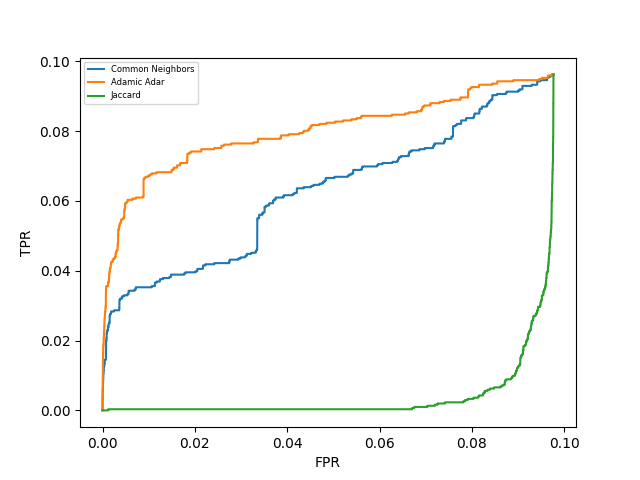
\includegraphics[width=0.45\textwidth]{img/linkPred/firstgraph.png}
    \caption{ROC curve of Jaccard, Adamic Adar and Common Neighbours}
    \label{fig:my_label}
\end{figure}

\begin{figure}[!htbp]
    \centering
    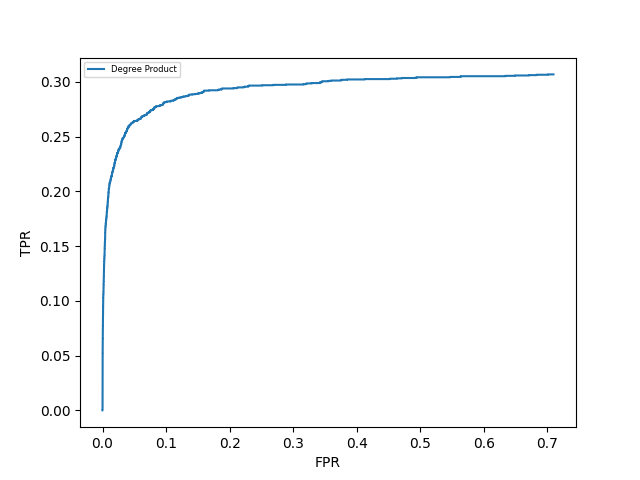
\includegraphics[width=0.45\textwidth]{img/linkPred/secondgraph.png}
    \caption{ROC curve of Preferential Attachment}
    \label{fig:my_label}
\end{figure}
As we can see, the Preferential attachment algorithm has an AUC orders of magnitude better than the rest.

\section{Task 4: open question}

The open question we chose concerns the degradaded use of public space by scientists in time of pandemic and the superficial behaviour of mainstream media. More precisely, the fundamental question is: have scientists been communicating for the public sake or, in contrast, for their own personal agenda? Moreover, we want to understand if mainstream media guaranteed equal weight and space to each expert, especially in public channels (as Fazio assures).
\subsection{Assumption}
During the Covid pandemic, TV shows have been more and more populated by scientists making their own claims in a climate of substantial chaos. These TV talks should have been a moment of clarity but, as the pandemic went on, chaos arose: a great part of these talks have been resembling a war between specialists that didn’t help the population at all, instigated by TV hosts in order to maximize their share. Despite their teacher role, some of these scientists chose to engage in “unprofessional ways”, led by the will to improve their own agency rather than by the will to actually help the population. In this way different niches arose on their affirmations, animating the public discourse on the internet. We decided to catch these niches by using Twitter because of its transversal use (both by masses and institutions). Taking an Oscar Wilde’s quotation from Dorian Gray as our reasoning basis:
\begin{quote}
    “There is only one thing in the world worse than being talked about, and that is not being talked about.”
\end{quote}
Starting from this affirmation, we chose a list of 13 well known italian scientists, selecting them on the basis of their growing popularity during the pandemic. We have done this with the intent to unveil the “influencer aspiration” of some of these scientists and the behaviour of certain TV shows in this dynamic. Watzlavick states as his 2nd communication axiom:
\begin{quote}
    “Every communication has a content and relationship aspect such that the latter classifies the former and is therefore a meta-communication”
\end{quote}
In our assumption, something serious but obvious has happened: the message content has been subordinated to the logic of virality, neglecting the importance of the pedagogic role of scientists (both in contents and way of communication). In contrast, this meta-communication dynamic reveals in scientists the same mistake often made by journalists: making scandalous claims on the basis of rumors, disguising hypotheses as ultimate truths while insulting others in the name of their own authority. In this case we can find a disruptive mix of both categories. We thus tried to address this problem through Network Science tools.



\subsection{Methods}
We decided to use the mention as link because of its clear semantic: mentioning someone is to appeal directly to him. During this process, all those with no mentions have been discarded. This has been done in order to create a significant lighter sample to facilitate either calculations and visualization.
As we said by quoting Wilde and Watzlavick, at this stage is not important the actual content of a message but its very existence. By doing this we are able to trace communities, considering a community as a group of indivdual that tend to mention the same individual. Thus we generated a weighted directed network and used Python for algorithm computation and, in the next section, we used it also for statistic visualization on sentiment analysis and date metadata.
To perform sentiment analysis (according to the limited power of our machines) we decided to filter data again, this time by italian language only and we deleted rows with repeated tweets (they were repeated because of the fact that a single user can mention multiple individuals within the same tweet and we derived a dataset just for mentions, thus we had several rows with the same communication index). The resulting dataset is composed by 68.000 rows. Coming to the method, we used “FEEL-IT” as a training dataset (available on Huggingface). Then we also split the results into 2 different dataframes according to the nature of tweets (positive or negative). As a final data manipulation we created 2 other types of dataframes starting from this last one and we made it for each subject of interest: one by username (i.e.: tweets TO others) and one by screen$\_$name (tweets received BY others). We decided also to create some wordclouds according to sentiment analysis, in order to visually catch the most frequent terms.

\subsection{ Network analysis results}
As we already said, our directed graph displays $\gamma = 2.39$ thus placing our network in the Scale-Free regime in which Ultra-Small World\cite{barabasiCh4.6} property ($2< \gamma <3$) is shown, as supported by the degree distribution which follows a clear power law. Due to the presence of hubs, in this regime the distances between nodes are drastically reduced. To better understand the role and the identity of these hubs we used some centrality measures. Between these ones, we would focus on two of them: PageRank (because it’s a variation of the Eigenvector centrality which is intended for weighted digraphs and thus considers weighted in-degree) and Closeness centrality (which yields as a result the easiest reachable node from any other node, reasoning on the sum of shortest paths).

Starting from PageRank we can clearly see that Capua’s score is the highest while Burioni’s is slightly lower, making him reach the 2nd position. The result diverges sligthly from our prediction because we hypothesized that Burioni would have been scoring always 1st. This could be consistent with the fact that even if Burioni has the highest weighted in-degree of the network, the nodes that connect to him are mostly uninfluential ones (e.g. uninfluential twitter users, probably trying to “blast the blaster”). Moreover, Burioni’s writing style avoids using mentions. In contrast, Capua has a stronger weighted out-degree than Burioni because she tends to mention often, especially influential nodes. This could be the reason of her highest score: in PageRank the most connected nodes are the most important and in this case she connects to higher in-degree nodes than Burioni. Going further in PageRank scores, as we expected, there are no other expert (aside from Zangrillo in the 6th position), instead we found self-referential organizations and a Rai3 TV show. More in detail: “onehealthuf” in 3rd position (One Health Center of Excellence, University of Florida, whose director is Capua),  “chetempochefa” in 4th position (Fazio’s tv show on Rai3, having Burioni as constant and privileged host even if Fazio denies it) and “medicalfactsit” in 5th position (whose founder and most active player is Burioni).  So reasoning about these scores we can see how  the most influential nodes according to PageRank are strongly interconnected. In this way the first 2 nodes saturate indirectly the top-5: one for Capua and two for Burioni (“Che Tempo Che Fa” did not host Capua at all or, if it is false, it has hosted her for an insignificant fraction of time compared to Burioni).
Coming to Closeness centrality, Burioni is 1st as he displays the lowest  value in the sum of shortest paths (thus an higher Closeness score), making him the node which can influence the entire network  quicker than others. This could be due to disproportionate Burioni’s weighted in-degree. Meanwhile, nodes in top 6 remain almost constant: Capua holds the 2nd place, “chetempochefa”  the 3rd one, Zangrillo the 4th one, “medicalfactsit” and “corriere” respectively 5th and 6th ones. This corroborates the PageRank results by adding to the most influential nodes also “Il Corriere della Sera”. But as we can observe, in this case the top 6 is saturated indirectly by Burioni (i.e.: “onehealthuf” disappears and “corriere” comes in while “chetempochefa” and “medicalfactsit” keep on displaying). Moreover, given both PageRank and Closeness scores, Zangrillo appears as an important player in discourses between/about experts in pandemics.

In the case of community discovery, a significant measure is given by the Angel algorithm score (we decided to use this because as we previously said it performs better in Internal Evaluation Strategies and it gives the best F1 score, tested against our ground truth). With a minimum community size equal to 9, it gave us 3 communities and this is significant because we can ascribe one to Burioni, one to Capua and the other one as a miscellaneous community composed by other experts plus the nodes connected to them (users or media).


\subsection{Sentiment analysis and chronological distribution}

\begin{figure}[htbp!]
  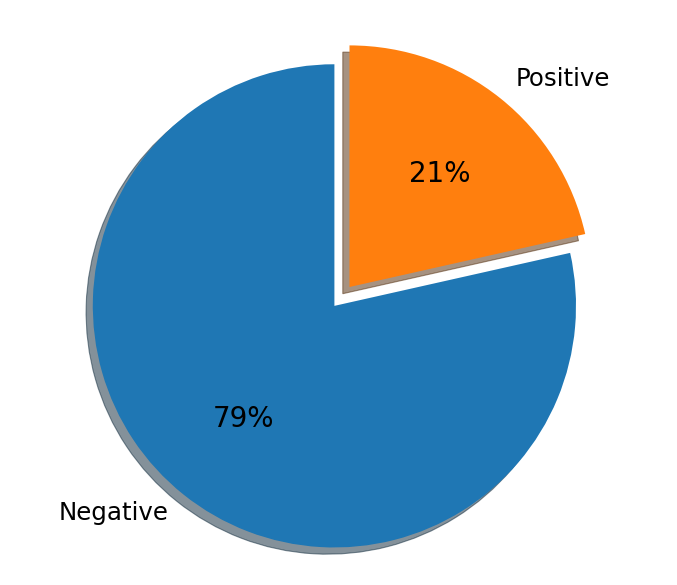
\includegraphics[width=.5\linewidth]{img/Results/SentimentAnalysis_pie.png}
  \captionof{figure}{Percentage of positive and negative tweets}
\end{figure}


The vast majority of tweets, as we expected, are negative. This means that population has been heavily polarized by the Covid-19 pandemic and this polarization led to a mutual aggressive behaviour. Reasoning about the intense activity of scientists across all media, one might think that this could have led to a more conscious and civil cultural democratic process but this, outrageously, is not the case: the population became more and more intolerant forgetting the fundamental respect that an healthy democracy requires.
\begin{figure}[htbp!]
  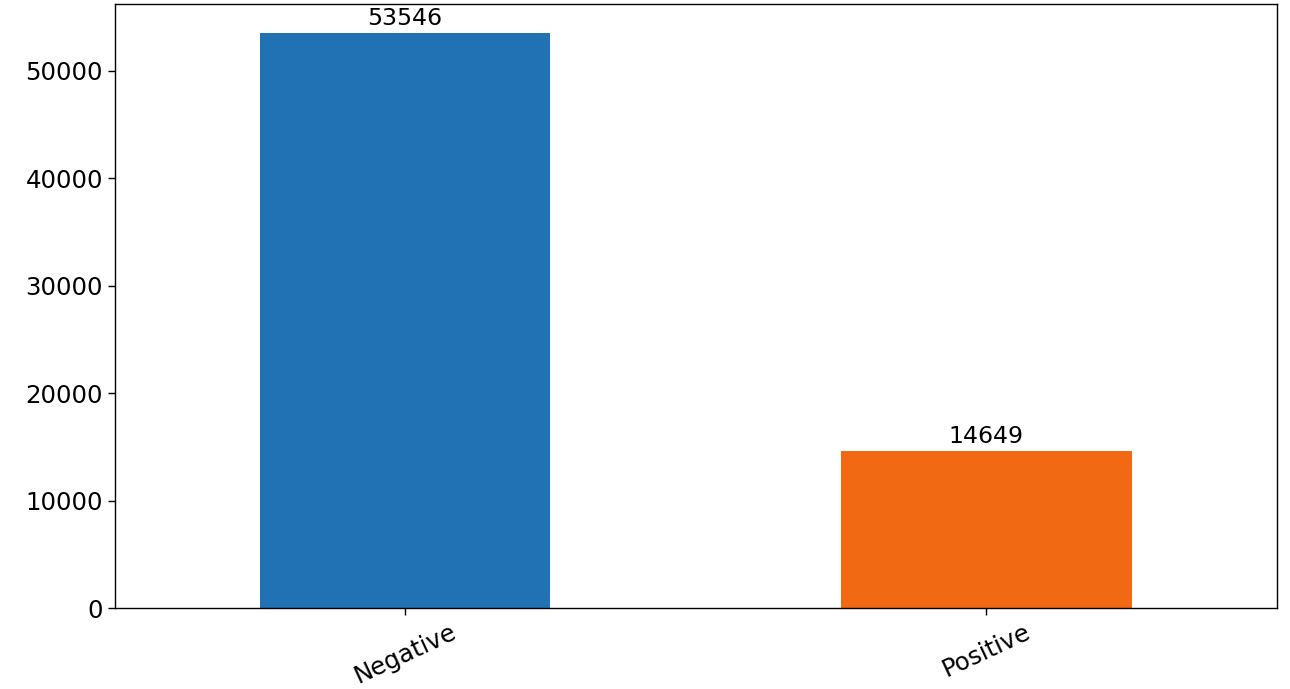
\includegraphics[width=.5\linewidth]{img/Results/SentimentAnalysis_histVal.png}
  \captionof{figure}{Absolute number of positive and negative tweets}
\end{figure}
If we assume that behaviour can also be modeled by observation and if we consider the influencing role of authorities, then we can state that the harsh and superficial behaviour between experts has been reflected onto the masses. This leads to a lack of understanding in the communication processes due to the lack of fine-tuning, turning places of public debates into hate forges. This negative dynamic, which is always quite natural also in peaceful times, has reached its peak in Italy right at the beginning of the perception of the pandemic and not at the very beginning of it. This is a clear sign of the importance of media coverage as event catalysts. As a matter of fact, in January there were already hidden institutional worries and meetings due to the pandemic plan which had not been updated since 2006. Then in February a broadcasted state propaganda started along with the emanation of the first Covid-19 driven D.P.C.M. .
\begin{figure}[htbp!]
\centering
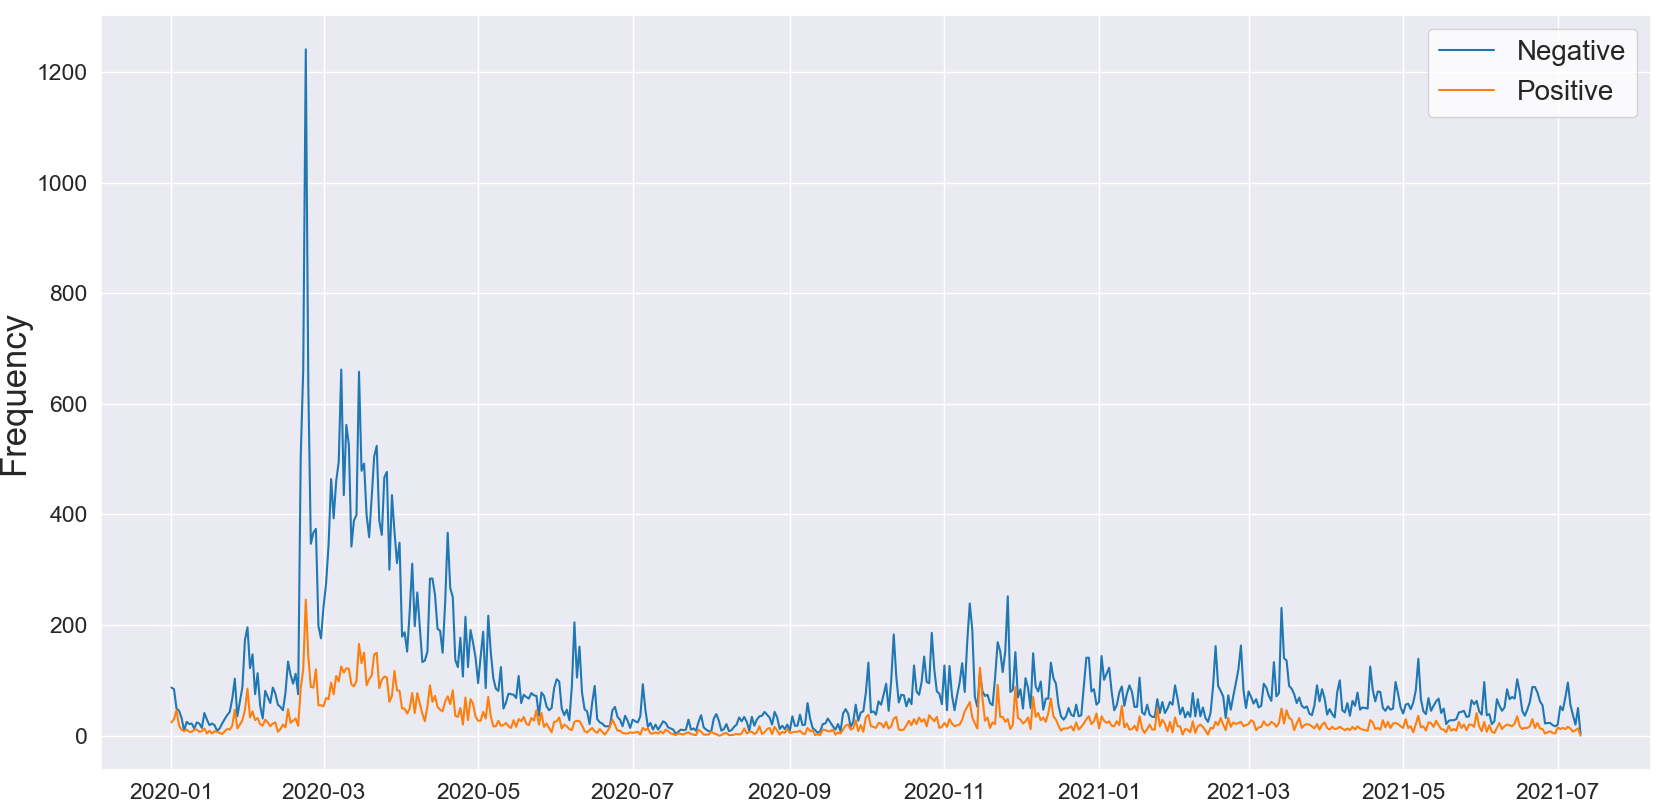
\includegraphics[width=.45\textwidth]{img/Results/SentimentAnalysis_line.png}
\captionof{figure}{Sentiment distribution according to time\\ (absolute values)}
\end{figure}

\begin{figure*}[!htpb]
    \centering
    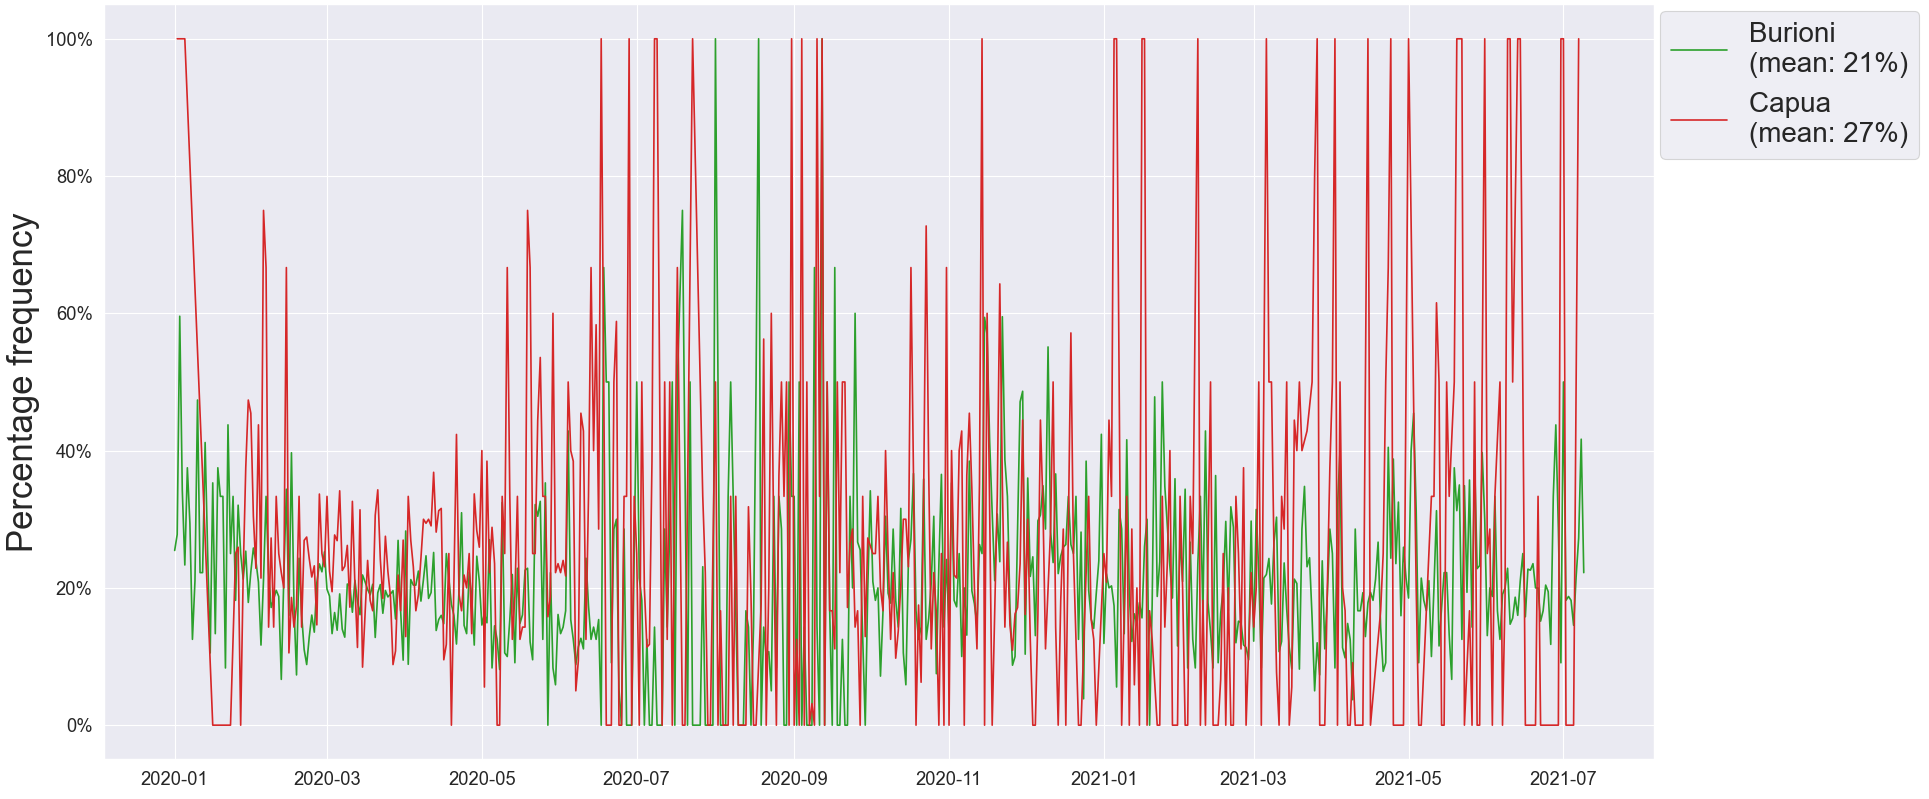
\includegraphics[width=\textwidth]{img/Results/comparison/Sentiment_screenname_Positive_perc_line(PT1).png}
    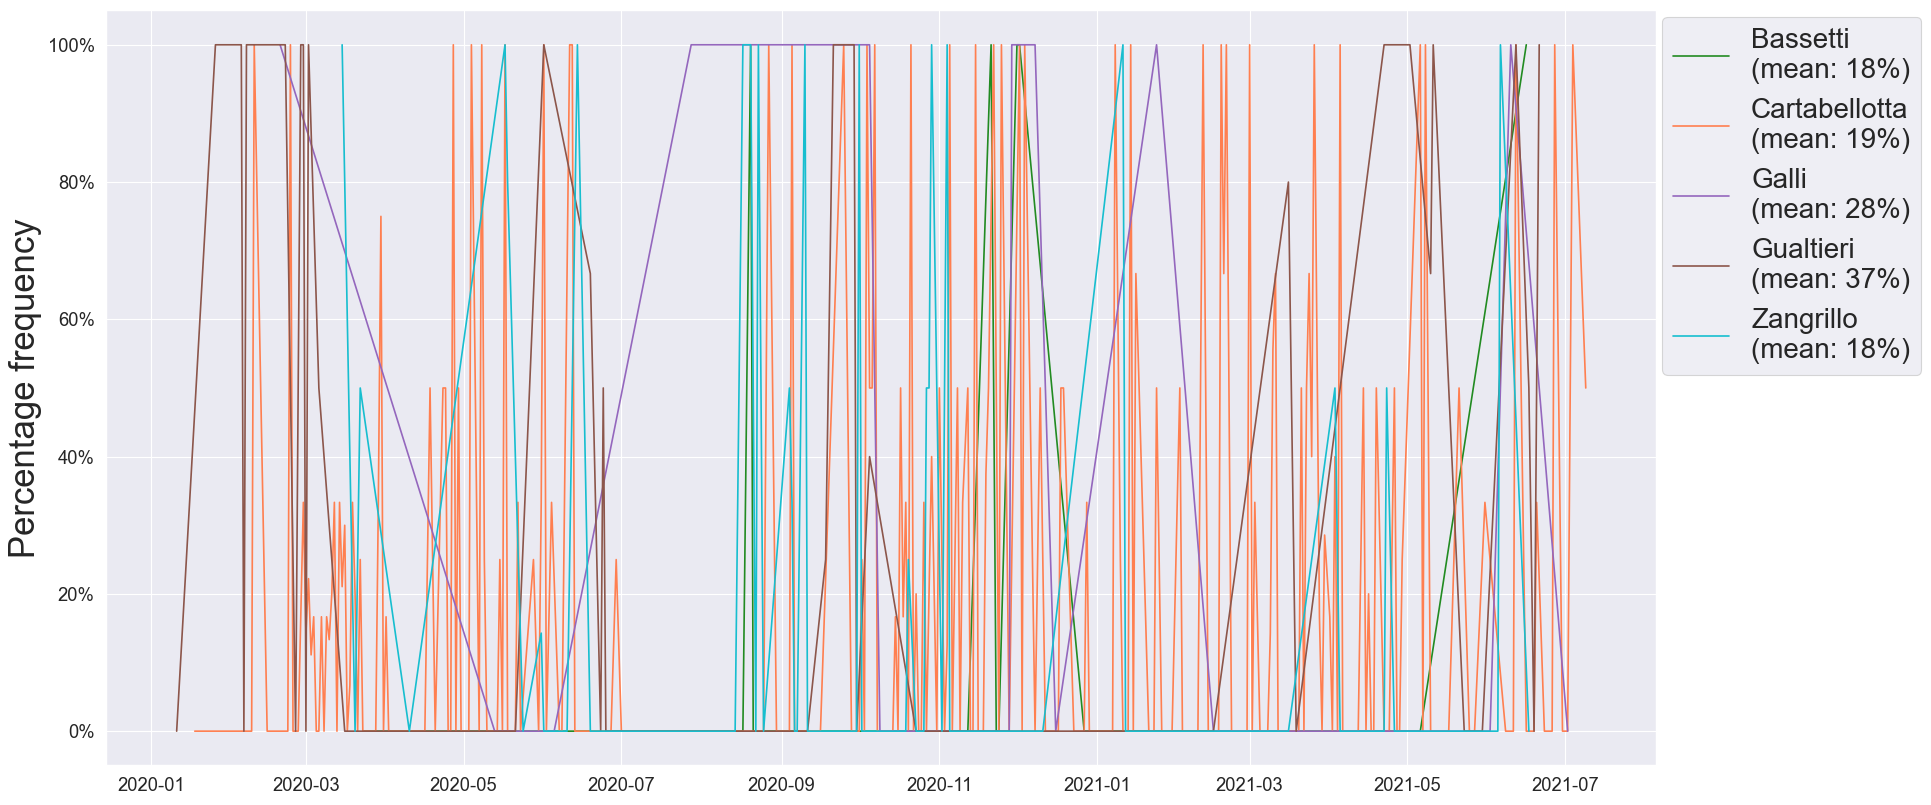
\includegraphics[width=\textwidth]{img/Results/comparison/Sentiment_screenname_Positive_perc_line(PT2).png}
    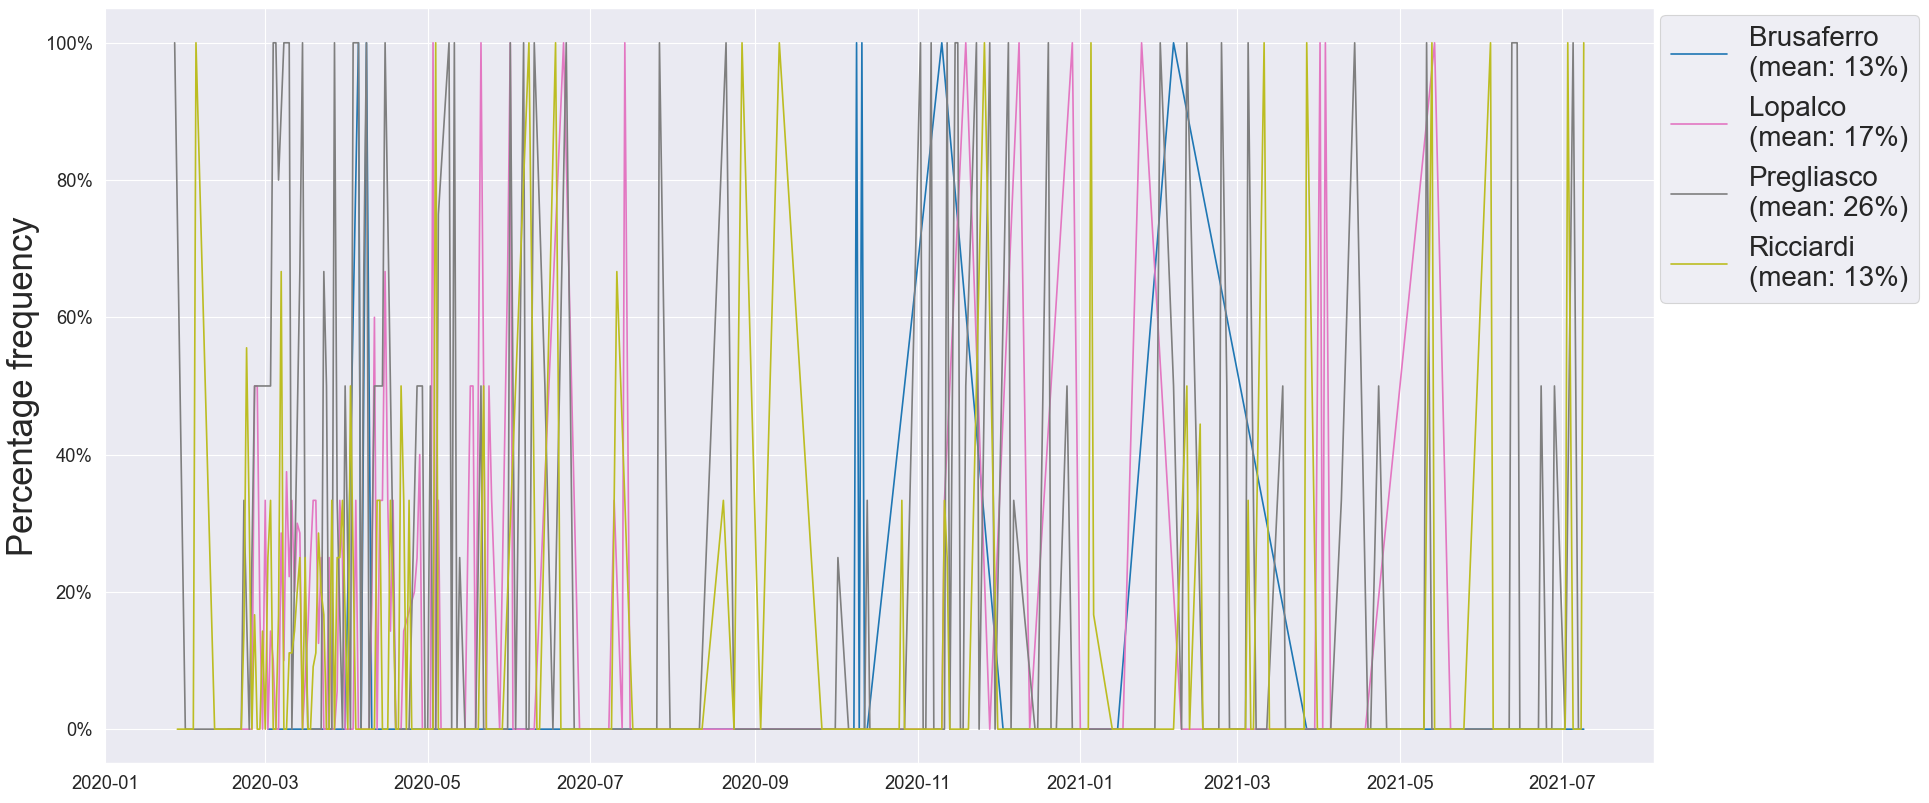
\includegraphics[width=\textwidth]{img/Results/comparison/Sentiment_screenname_Positive_perc_line(PT3).png}
    \caption{Personal positive sentiment distribution percentage per day (received tweets only)}
\end{figure*}


In this event, the population has been witnessing the saturation of virtual public spaces by politicians and experts. The constant coverage about the topic made by them had, since start, a disruptive outcome on the population. This resulted on more confusion and thus on a more sensationalistic overall tone, inducing masses to disinformation. This is a sign of the damages caused by top-down (subtle) impositions: information appears as knowledge but there cannot be knowledge only by passive information. Reflective information is the very core of an healthy democracy but mainstream media induce often, like in this case, to the opposite effect: population does not feel obliged to reflectively search about things because, common thought, what is important is already said by mainstream media. This is indeed a vicious circle, a vicious circle that has been amplified in time of disaster.

Observing the line plot we can see how peaks (both positives and negatives) anticipate or follow each other, giving the idea of individuals constantly fighting for each important event (from experts statements to D.P.C.M emanation). As the graph suggests, there is a first little peak in the 2020/01/31. The day before the state of emergency had been proclaimed by the Council of Ministers, after weeks of confidential meetings\cite{regioni}. The true peak is reached on 2020/02/23, the day in which the first D.P.C.M. was emanated\cite{dpcm}. From this date to 2020/08 we can observe a slow decline in the users activity (followed by a summer pause which we’ll comment later on). Then, other three minor peaks can be observed:
\begin{itemize}
    \item 	two contained between the start of 2020/10 and the start of 2020/12 %
    (2020/10/10 ; 2020/11/26);
    \item 	the other contained between the end of 2021/02 and the end of 2021/03 %
    (2021/03/14);
\end{itemize}

To better understand the nature of these peaks, we derived two more graphs (one for negative mentions done to someone and one for positive ones), plotting lines from crosstabs for each influential-expert on twitter (so not all 13 due to lack of data) to understand who has been playing a crucial role for the biggest peak.
\begin{minipage}{0.5\textwidth}
\centering
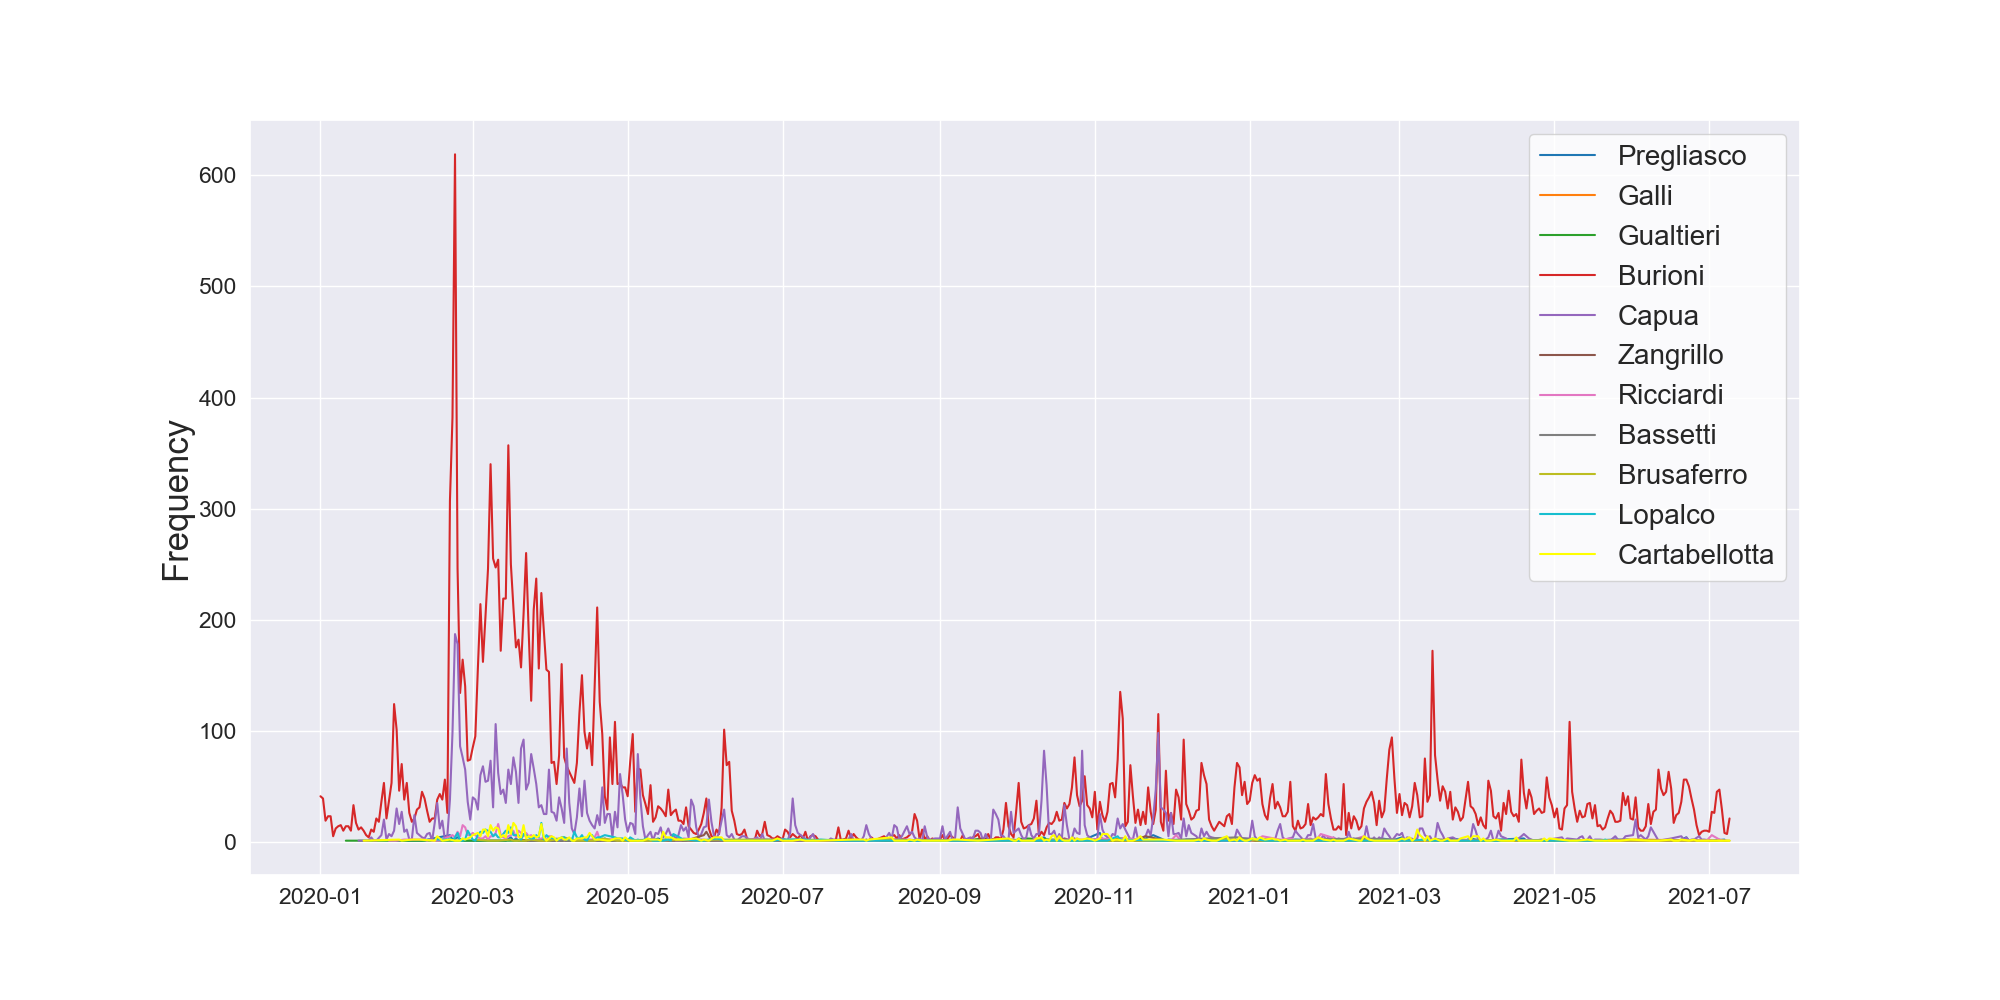
\includegraphics[width=\textwidth]{img/Results/comparison/Sentiment_screenname_Negative_line.png}
\captionof{figure}{\\Personal negative sentiment distribution according to time\\ (received tweets only)}
\end{minipage}
\begin{minipage}{0.5\textwidth}
\centering
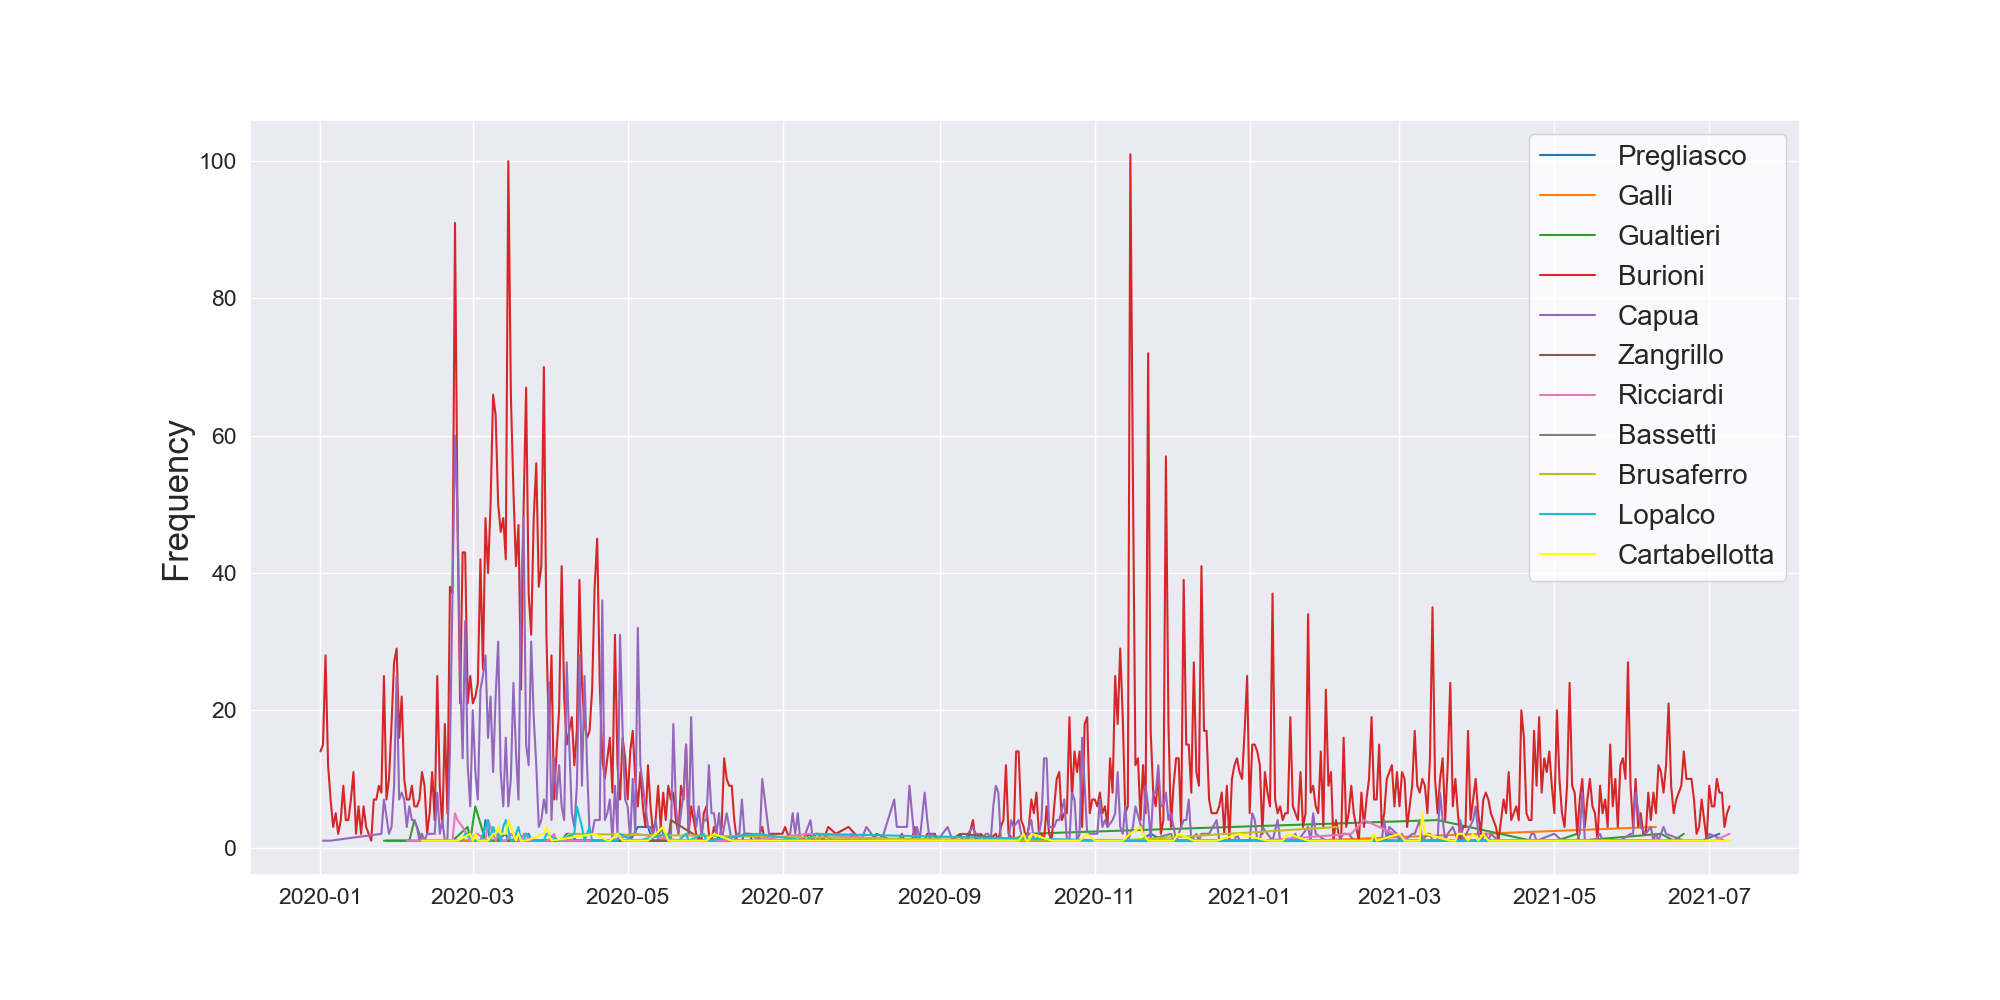
\includegraphics[width=\textwidth]{img/Results/comparison/Sentiment_screenname_Positive_line.png}
\captionof{figure}{\\Personal positive sentiment distribution according to time\\ (received tweets only)}
\end{minipage}
\\ \\
Given the comparison between individual trends, we can assume that major peaks are due to Burioni’s activity. We can conclude so because, as can be observed, others experts’s activities remain almost constant in time, Capua excluded. Moreover, dividing the observation according to years, Capua’s activity is important during the very beginning of the pandemic, becoming more and more irrelevant as time passes. This irrelevance becomes more noticeable after 2020’s summer, when Burioni comes back to polarize the debate.
 As we said before, the summer pause seems quite significant. This insight is corroborated by the fact that Burioni effectively has a major role on the general trend. As a matter of fact, that pause overlaps with Burioni’s self-imposed media blackout, “at least until Autumn” he said\cite{corriereB}. Meanwhile, he kept on posting on his own pages (also ‘medfactsit’). This media blackout starts on 2020/06/08 and as we can see in either positive or negative tweets received, the last red peak falls on this exact date. This event has been producing more negative tweets than positive ones (100 negatives against less than 20 positives).

 After the summer pause, in which Capua becomes the most active player, the gradual increase in Burioni’s trend leads to another important peak in which negative and positive comments are almost equal (less than 150 negative and 100 positives). This peak, as we said, happens on the 2020/10/10 and this date overlaps with a controversial tweet made by Burioni\cite{fattoQuot}. Again, the peak observed on the 2020/11/26 could be due to the controversy happened between Capua and Burioni the day before\cite{burioni}. Going further with the interpretation of this summer pause, focusing on Burioni’s activity, a critical insight can be reached on the trend activity: a clear descent can be noticed during May 2020 and a following ascent happens at the end of September 2020. Considering that, since the very beginning of experts exposition on TV shows, Che Tempo Che Fa chose Burioni as a scientific testimonial (hosting him each and every Sunday) and considering that the end of the 2019-2020 season happened on Sunday 23 May while the 2020-2021 season started on Sunday 27 September, a clear date overlapping can be observed. Given this observations, we can assume that Che Tempo Che Fa has been the niche in which Burioni gained more fame than ever (between masses of course).
 \\
 Finally, three wordclouds (total, positive, negative) are given in order to visualize the most frequent words.
  \begin{figure}[!htbp]
 \centering
 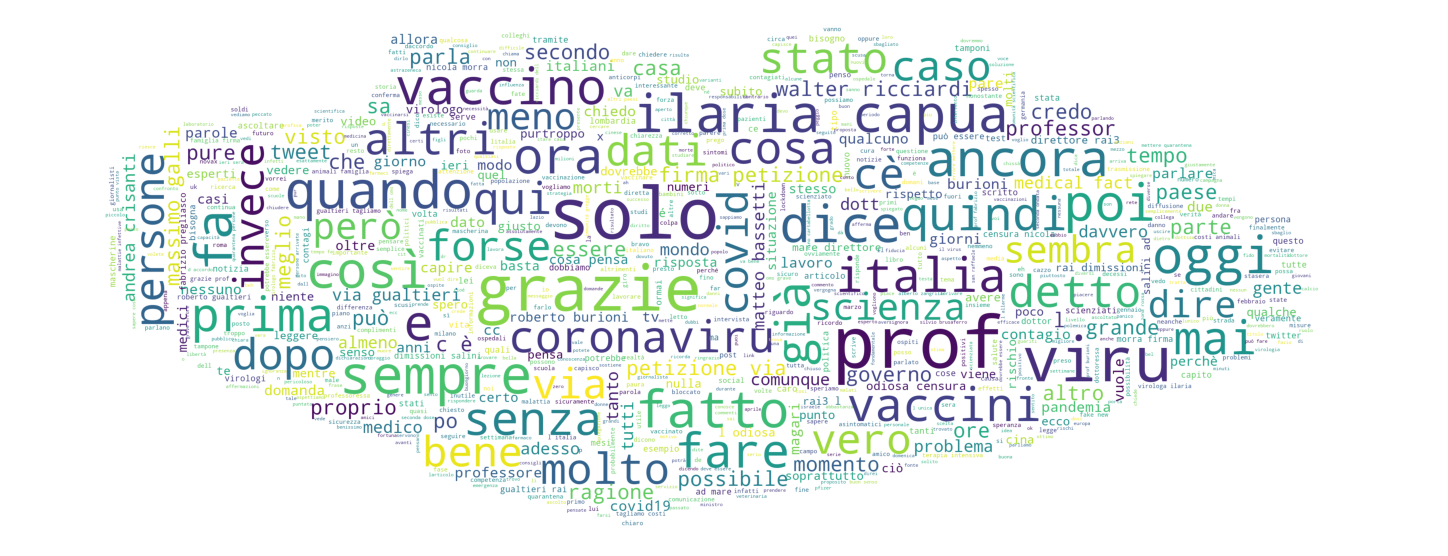
\includegraphics[width=0.50\textwidth]{img/Results/Wordclouds/Sentiment_All_Wordcloud.png}
 \caption{Complessive wordcloud}
 \end{figure}

 \begin{figure}[!htpb]
 \centering
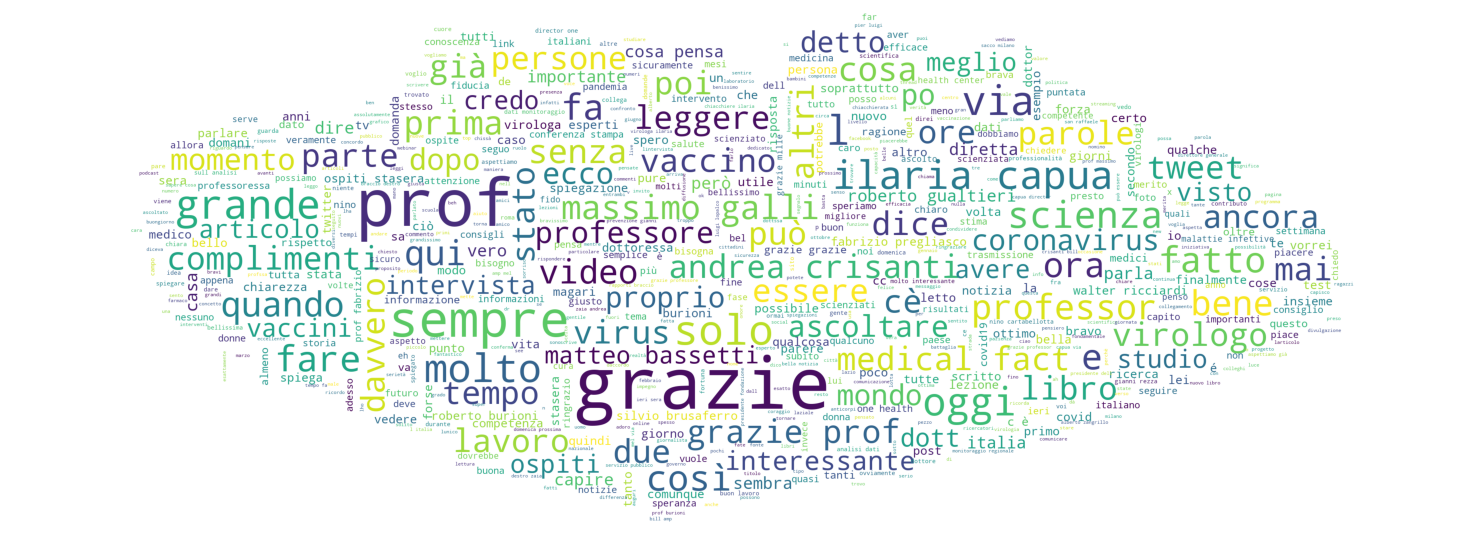
\includegraphics[width=0.45\textwidth]{img/Results/Wordclouds/Sentiment_Positive_Wordcloud.png}
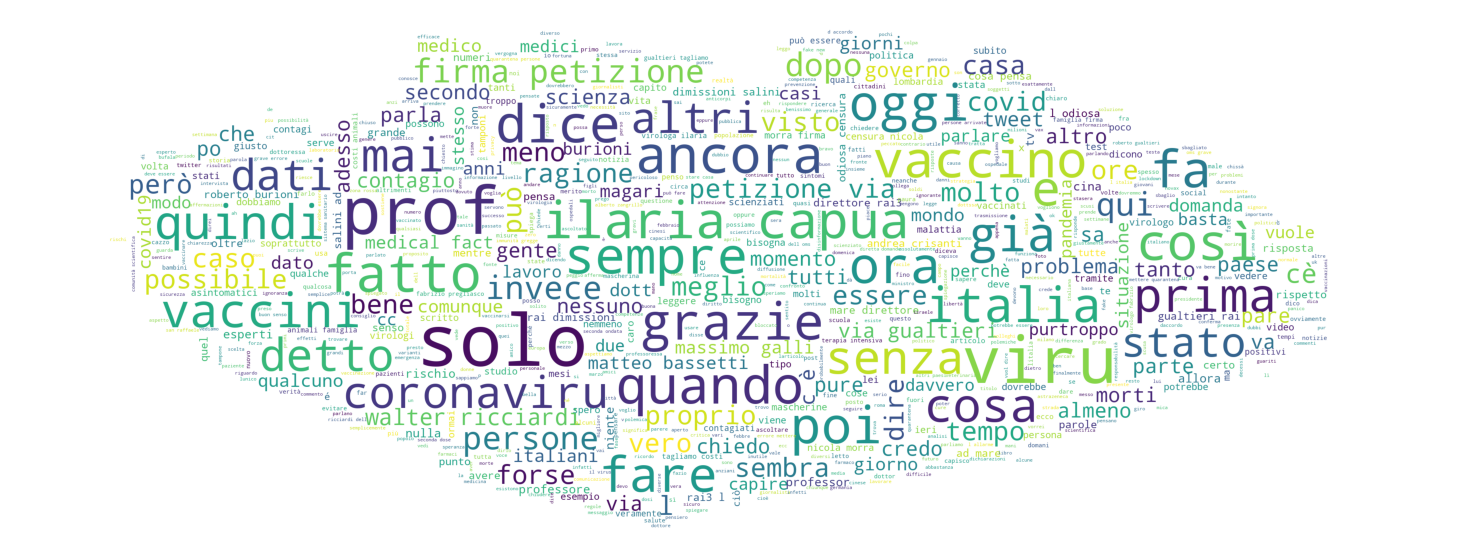
\includegraphics[width=0.45\textwidth]{img/Results/Wordclouds/Sentiment_Negative_Wordcloud.png}
\caption{Positive vs Negative wordcloud}
    \label{fig:my_label}
\end{figure}
\bibliographystyle{ACM-Reference-Format}
\bibliography{biblio}
\end{document}